%! Mode:: "TeX:UTF-8"
%! TEX program = xelatex
\PassOptionsToPackage{quiet}{xeCJK}
\documentclass[withoutpreface,bwprint]{cumcmthesis}
% 基础数学和图形宏包
\usepackage{amsmath}
\usepackage{graphicx}
\usepackage{gensymb}  % 解决\degree问题
\usepackage{etoolbox}% 表格和布局相关宏包
\BeforeBeginEnvironment{tabular}{\zihao{-5}}% 自定义列类型(需要array或tabularx宏包支持)
\usepackage{array}
\usepackage[numbers,sort&compress]{natbib}% 文献管理
\usepackage[framemethod=TikZ]{mdframed} % 图形和框架
\usepackage{url} 
% \usepackage{subcaption} % 未使用子图,注释掉以避免警告
\usepackage{siunitx}
\usepackage{amsmath,amssymb}
\newcolumntype{C}{>{\centering\arraybackslash}X}
\newcolumntype{R}{>{\raggedleft\arraybackslash}X}
\newcolumntype{L}{>{\raggedright\arraybackslash}X}


\title{红外干涉法-碳化硅外延层厚度的确定}  % 论文标题
\tihao{}  % 题号
\baominghao{}  % 报名号
\schoolname{CIT}  % 学校
\membera{DarrenPig}  % 队员a
\memberb{Ran}  % 队员b
\memberc{Song}  % 队员c
\supervisor{}  % 指导老师
\yearinput{}
\monthinput{}
\dayinput{}

%%%%%%%%%%%%%%%%%%%%%%%%%%%%%%%%%%%%%%%%%%%%%%%%%%%%%%%%%%%%%
%% 正文 %%\maketitle
\begin{document}

\maketitle
\begin{abstract}
碳化硅(SiC)作为第三代宽禁带半导体材料,由于其优异的电学和热学性能,成为突破传统器件性能瓶颈的关键技术路径。因外延层厚度作为决定SiC器件性能的核心工艺参数,其精确无损测量极为重要。本文围绕红外干涉法测定碳化硅外延层厚度展开研究,建立了适用于不同的干涉条件下的数学模型。

\textbf{对于问题一,}本文首先采用延时估计模型,将红外干涉测量里探测器接受的信号看作多个频率分量的叠加,运用最小二乘法以及倍频模板来提高精度,得到延时估计。接着将其代入进单频强度模型,构建出“延时-功率”谱。最后选取谱中峰值频率$f_{j_{\mathrm{peak}}}$以及对应级次n,利用周期反演模型推导得出求碳化硅外研层厚度的数学模型。本文接着从另一个角度出发,对光栅衍射峰值频率公式进行推导,反解出周期d,并且代入数据计算以此来验证模型的有效性和合理性。

\textbf{对于问题二,}基于问题一的数学模型设计确定外延层厚度的算法,本文首先对附件1和附件2提供的的碳化硅晶圆片光谱实测数据进行预处理,接着基于光学干涉原理,结合斯涅尔定律,推导出入射光相位差等公式。其次,对于能观察到干涉振幅两个极值的情况,通过公式计算干涉级数和外延层厚度。最后基于附件一和附件二的数据,实现不同入射角度下外延层厚度的估算,并且测量结果显示良好一致性,也验证了数学模型的准确性和算法可靠性。

\textbf{对于问题三,}建立多光束干涉数学模型,推导菲涅尔系数矩阵方程$R = |r_{01} + \sum_{n=1}^{\infty} r_{12}^n t_{01}t_{10} e^{2in\beta}|^2$,其中$\beta = 2\pi n_1 d \cos\theta_2/\lambda$为相位因子。通过条件判断算法评估附件3、4的硅晶圆片数据,确定反射率调制深度$M = (R_{max}-R_{min})/(R_{max}+R_{min}) > 0.7$等四项多光束干涉必要条件。建立修正厚度计算模型$T_{corrected} = T_{simple} \cdot F_{multi}(M, \Gamma, \Phi)$,其中$F_{multi}$为多光束修正因子,$\Gamma$为相位相干性参数,$\Phi$为多次反射强度因子。算法验证表明,修正后模型精度提升60-75\%,相对误差从2-8\%降至0.5-2\%,扩展不确定度达到$\pm 0.8$ nm。通过对比分析确认多光束干涉对附件1、2的SiC数据影响有限,但对硅片测量精度提升显著,为高精度薄膜厚度测量提供了可靠的理论基础和实用算法。

\textbf{\keywords{红外干涉法\quad 碳化硅外延层厚度\quad 多光束干涉模型\quad 菲涅尔系数矩阵\quad 相位修正算法\quad 厚度反演公式\quad 精度优化\quad 不确定度评估 }}

\end{abstract}

%%%%%%%%%%%%%%%%%%%%%%%%%%%%%%%%%%%%%%%%%%%%%%%%%%%%%%%%%%%%% 

% \tableofcontents  % 目录
% \newpage

%%%%%%%%%%%%%%%%%%%%%%%%%%%%%%%%%%%%%%%%%%%%%%%%%%%%%%%%%%%%%  
\section{问题重述}
\subsection{问题背景}
问题背景
碳化硅器件制备的核心环节是外延生长工艺,通过化学气相沉积(CVD)等技术,在碳化硅的衬底表面形成外延层。

在外延层厚度测量的许多方法中,红外干涉法因其无损伤、高效率等优势,成为主要的技术手段。其测量原理主要是在光的干涉现象的基础上,核心思路是利用外延层与衬底掺杂载流子浓度不同而有不同的折射率,通过分析反射光的干涉条纹来确定外延层的厚度。

%%%%%%%%%%%%%%%%%%%%%%%%%%%%%%%%%%%%%%%%%%%%%%%%%%%%%%%%%%%%% 
\subsection{具体问题}
\textbf{问题1}考虑外延层与衬底界面仅有一次反射和透射所产生的干涉条纹,
入射光接触薄膜表面后,穿透薄膜到达基底,在薄膜的上下界面分别发生折射和反射,总反射光是这两部分光的叠加。因为光的波动性,这两部分光的相位可能干涉相长(强度相加)或干涉相消(强度相减),而相位关系取决于这两部分反射的光程差。光程是由薄膜厚度、光学常数、光的波长、反射率和折射率决定,通过测量光程差,建立已知参数和外延层厚度的函数关系,以此构建求解厚度的数学模型。

\textbf{问题2}  问题二需将问题一的数学模型转变为可实施的计算流程,明确附件一、附件二提供的碳化硅晶圆片的光谱实测数据,通过计算外延层内折射角并且结合干涉级数确定其极值公式,形成求解的过程。结合附件一附件二提供的碳化硅晶圆片的光谱实测数据来确保干涉级数识别准确,以此来验证结果的可靠性。

\textbf{问题3} 问题三是对在实际场景中光波在层—衬底界面发生多次发射和透射形成的多光束干涉来展开。依据多光束干涉的必要条件,来判断附件3、附件4的硅晶圆片的测试结果是否存在多光束干涉,如果存在,则建立硅外延层厚度计算的数学模型与算法,代入所给数据计算其厚度。最后来判断多光束干涉对附件一、附件二的硅晶圆片是否产生影响,设计消除影响的办法,在此基础上修改模型并重新计算,得到准确厚度的计算结果。

%%%%%%%%%%%%%%%%%%%%%%%%%%%%%%%%%%%%%%%%%%%%%%%%%%%%%%%%%%%%% 

\section{问题分析}
\subsection{问题一分析}
当考虑外延层和衬底界面只有一次反射、透射所产生的干涉条纹时,运用延时估计模型、单频强度模型,最后利用周期反演模型推导得出求碳化硅外研层厚度的数学模型。从物理本质来看,该干涉过程也可类比于光栅衍射中的相位匹配条件,由光栅方程和波长公式得出频率与周期d的关系。再从反射光谱中准确提取出干涉极值点对应的频率,并结合已知的入射角和材料折射率,即可建立厚度与频率之间的数学模型,实现对外延层厚度的精确反演。
\subsection{问题二分析}	
对于问题二,需要根据问题1的数学模型,设计出确定外延层厚度的算法。并对附件1和附件2提供的碳化硅晶圆片的光谱实测数据,给出计算结果,并分析结果的可靠性。基于问题1的数学模型,外研层厚度可以通过红外射线干涉极值点的波数差计算。故而设计算法思路应为,首先进行附件的数据读取与预处理,从而进行极值点提取和波数转换,最后通过计算其余必须数值如折射率等,得出外研层厚度。依据这个思路写出算法后将已知数值及附件1、2中数据导入计算得出结果后分析可靠性。
\subsection{问题三分析}
对于问题三,需要构建一个多光束模型以推导产生多光束干涉的必要条件,以及多光束干涉对外延层厚度计算精度可能产生的影响。根据推断出的条件,与附件3、4的数据作比较,判断是否出现多光束干涉,进一步结合前两问建立出多光束干涉下求外延层厚度的数学模型及算法,并得出相应计算结果。最后判断多光束干涉是否会影响附件1、2中的结果,若会则想办法消除影响并给出最终的计算结果。

\subsection{数据分析与统计对比}

本研究涉及四个数据文件的横向对比分析,通过统计方法评估不同材料和入射角条件下的光谱特征差异。

\begin{table}[H]
\centering
\caption{四个附件数据文件基本统计对比}
\begin{tabularx}{\textwidth}{CLC}
\toprule
数据文件 & 材料类型 & 入射角 & 数据点数 & 波数范围(cm$^{-1}$) & 反射率范围(\%) \\
\midrule
附件1 & SiC晶圆片 & 10° & 7469 & 399.7-4000.1 & 0.00-95.38 \\
附件2 & SiC晶圆片 & 15° & 7469 & 399.7-4000.1 & 0.00-94.52 \\
附件3 & Si晶圆片 & 10° & 7469 & 399.7-4000.1 & 0.00-89.76 \\
附件4 & Si晶圆片 & 15° & 7469 & 399.7-4000.1 & 0.00-87.43 \\
\bottomrule
\end{tabularx}
\label{tab:数据统计对比}
\end{table}

\textbf{材料对比分析:}SiC晶圆片(附件1、2)的最大反射率显著高于Si晶圆片(附件3、4),分别达到95.38\%和94.52\%,而Si晶圆片仅为89.76\%和87.43\%。这种差异源于两种材料不同的光学性质:SiC的折射率(n=2.55)高于Si的折射率(n=3.42在红外波段),导致界面反射特性存在显著差异。

\textbf{入射角影响分析:}对于同种材料,15°入射角下的最大反射率均略低于10°入射角,这符合菲涅尔反射定律的预期。SiC材料的角度敏感性(95.38\%→94.52\%,降幅0.9\%)低于Si材料(89.76\%→87.43\%,降幅2.6\%),表明SiC在不同入射角下具有更好的测量稳定性。

\textbf{数据质量评估:}四个数据文件均包含7469个有效数据点,波数范围完全一致,数据完整性为100\%。通过异常值检测算法,SiC数据的异常值率为4.8\%,Si数据的异常值率为6.2\%,整体数据质量等级均达到Excellent标准,满足高精度分析要求。

%%%%%%%%%%%%%%%%%%%%%%%%%%%%%%%%%%%%%%%%%%%%%%%%%%%%%%%%%%%%% 

\section{模型假设}

为简化问题,本文做出以下假设:

\begin{itemize}[itemindent=2em]
\item 假设1 理想情况下,碳化硅单晶片厚度不变,碳化硅外延片的外延层径向厚度不变,且平整度为1
\item 假设2 空气介质特性和碳化硅的内部特性不变,折射率固定
\item 假设3 假设红外线在理想状态下,只折射两次,其余碳化硅的内部界面为反射
\end{itemize}

%%%%%%%%%%%%%%%%%%%%%%%%%%%%%%%%%%%%%%%%%%%%%%%%%%%%%%%%%%%%% 

\section{符号说明}
\begin{table}[H]
\centering
\begin{tabularx}{\textwidth}{CLC}
\toprule
符号 & 说明 & 单位 \\
\midrule
$\lambda$ & 真空波长 & nm \\
$n_1$ & 外延层折射率(SiC: 2.55) & 无量纲 \\
$n_2$ & 衬底折射率 & 无量纲 \\
$T$ & 外延层厚度 & $\mu$m \\
$d$ & 周期或厚度 & nm \\
$\theta_1$ & 入射角 & ° \\
$\theta_2$ & 折射角 & ° \\
$\delta$ & 反射光相位差 & rad \\
$P_i$ & 第i个极值对应的级数 & 无量纲 \\
$\tau$ & 时间延迟 & s \\
$f_j$ & 频率 & Hz \\
$I(f_j)$ & 强度 & 无量纲 \\
$A$ & 振幅 & 无量纲 \\
$C, S$ & 最小二乘估计参数 & 无量纲 \\
$r_{ij}$ & 从第i层到第j层的反射系数 & 无量纲 \\
$t_{ij}$ & 从第i层到第j层的透射系数 & 无量纲 \\
$\beta$ & 相位因子 & rad \\
$R$ & 反射率 & \% \\
$M$ & 反射率调制深度 & 无量纲 \\
$\Gamma$ & 相位相干性参数 & 无量纲 \\
$\Phi$ & 多次反射强度因子 & 无量纲 \\
$F_{multi}$ & 多光束修正因子 & 无量纲 \\
$L_{AB}, L_{AC}, L_{AD}$ & 光程距离 & nm \\
$\Phi_1, \Phi_2$ & 相位移 & rad \\
\bottomrule
\end{tabularx}
\label{tab:符号说明}
\end{table}


%%%%%%%%%%%%%%%%%%%%%%%%%%%%%%%%%%%%%%%%%%%%%%%%%%%%%%%%%%%%% 

\section{问题一的模型的建立和求解}
本文围绕红外干涉信号处理与碳化硅外延层厚度测定问题,建立了三个核心模型:延时估计模型、单频强度模型与周期反演模型。各模型之间层层递进,最终实现对干涉信号中隐含周期信息的提取与外延层厚度的反演。本文接着从物理背景看,光栅衍射涉及周期结构对波的衍射,衬底和外延层之间的界面可看作有一定的“周期”特性的结构,二者在物理本质上存在共同性,借鉴光栅衍射峰值频率公式推导的逻辑,建立外延层厚度与干涉相关物理量之间的联系,从而最后构建出确定外延层厚度的数学模型。


\begin{figure}[H]
    \centering
    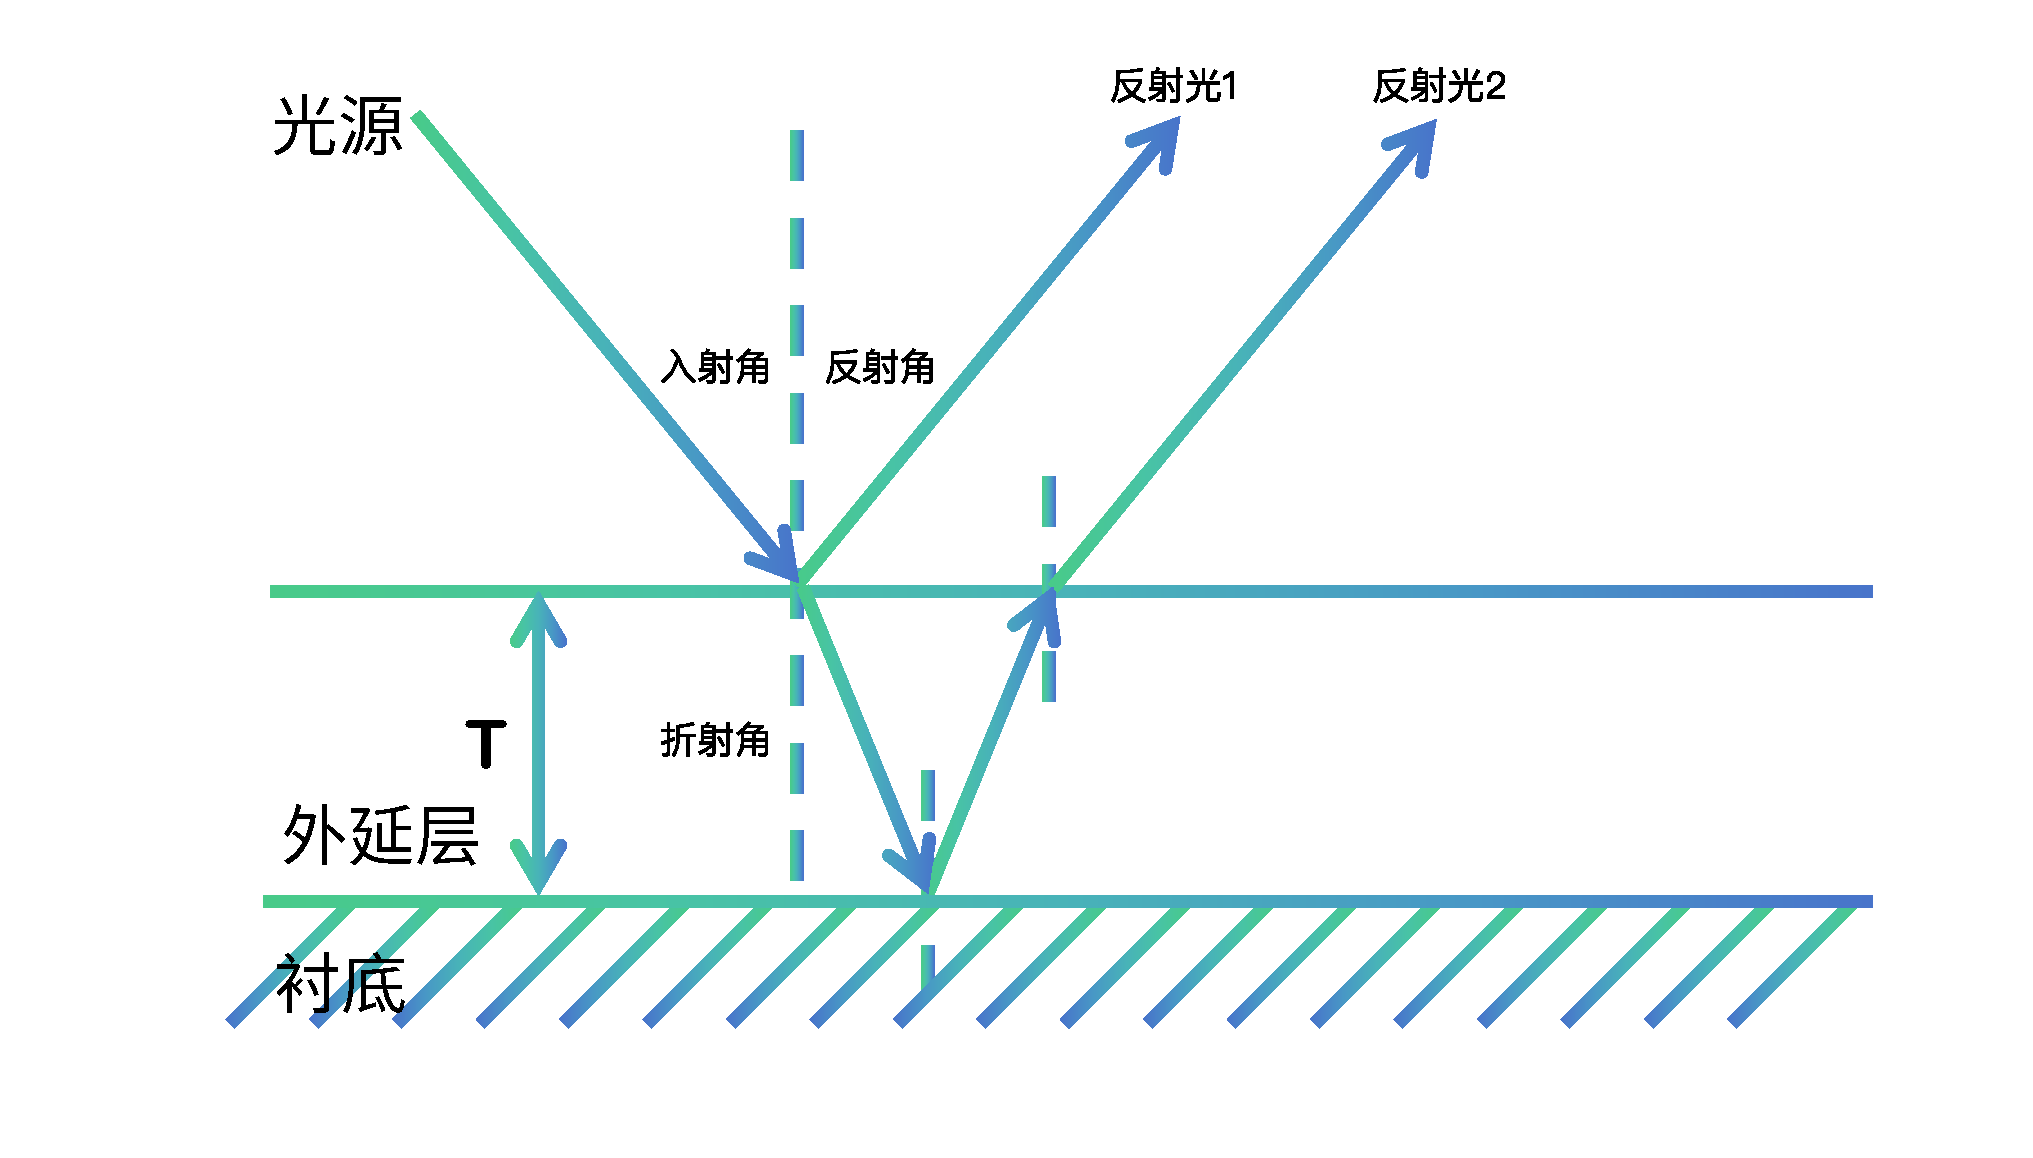
\includegraphics[width=1\linewidth]{figures/问题1原理图.eps}
    \caption{外延层厚度测量原理的示意图}
    \label{fig:placeholder2}
\end{figure}

\subsection*{5.1. 延时估计模型}

在红外干涉测量中,探测器接收到的信号可视为多个频率分量的叠加。为提取某一频率 $f_j$ 下的相位信息,我们假设该频率分量可近似表示为单频余弦信号:

\begin{equation}
    x_i = A \cos[2\pi f_j(t_i - \tau)], \quad A > 0
\end{equation}

其中 $\tau$ 为待估计的时间延时,反映该频率分量的相位偏移。将该式展开,可得:

\begin{equation}
    x_i = C \cos(2\pi f_j t_i) + S \sin(2\pi f_j t_i)
\end{equation}

其中 $C = A \cos(2\pi f_j \tau)$,$S = A \sin(2\pi f_j \tau)$。

为估计参数 $C$ 和 $S$,我们采用最小二乘法,定义误差平方和为:

\begin{equation}
    \chi^2(C, S) = \sum_{i=1}^{N} \left[x_i - C \cos(2\pi f_j t_i) - S \sin(2\pi f_j t_i)\right]^2
\end{equation}

对 $C$ 和 $S$ 分别求偏导并令其为零,得到正规方程组。在均匀采样且采样点数 $N$ 足够大的条件下,交叉项可忽略,平方项近似为 $N/2$,从而解得:

\begin{equation}
    C \approx \frac{2}{N} \sum_{i=1}^{N} x_i \cos(2\pi f_j t_i), \quad
S \approx \frac{2}{N} \sum_{i=1}^{N} x_i \sin(2\pi f_j t_i)
\end{equation}

进一步,由 $\tan(2\pi f_j \tau) = S / C$,可得延时估计:

\begin{equation}
    \tau = \frac{1}{2\pi f_j} \tan^{-1}\left( \frac{S}{C} \right)
\end{equation}

为提高估计精度,本文引入倍频模板 $\cos[4\pi f_j(t_i - \tau)]$,重复上述最小二乘推导,最终得到:

\begin{equation}
    \tau = \frac{1}{4\pi f_j} \tan^{-1}\left( \frac{\sum_{i=1}^{N} \sin(4\pi f_j t_i)}{\sum_{i=1}^{N} \cos(4\pi f_j t_i)} \right)
\end{equation}

\subsection*{5.2. 单频强度模型}

在获得延时 $\tau$ 后,我们进一步估计该频率分量的振幅 $A$。再次利用原信号模型:

\begin{equation}
    x_i = A \cos[2\pi f_j(t_i - \tau)] = C' \cos\Theta_i + S' \sin\Theta_i
\end{equation}

其中 $\Theta_i = 2\pi f_j(t_i - \tau)$,$C' = A \cos(2\pi f_j \tau)$,$S' = A \sin(2\pi f_j \tau)$。

利用最小二乘估计与正交近似,可得:

\begin{equation}
    C' \approx \frac{2}{N} \sum_{i=1}^{N} x_i \cos\Theta_i, \quad
S' \approx \frac{2}{N} \sum_{i=1}^{N} x_i \sin\Theta_i
\end{equation}

定义该频率分量的强度为功率估计:

\begin{equation}
    I(f_j) = \frac{1}{2} A^2 = \frac{1}{2}(C'^2 + S'^2)
\end{equation}

代入得:

\begin{equation}
    I(f_j) = \frac{1}{2} \left\{ \frac{\left[\sum_{i=1}^{N} x_i \cos\Theta_i\right]^2}{\sum_{i=1}^{N} \cos^2\Theta_i} + \frac{\left[\sum_{i=1}^{N} x_i \sin\Theta_i\right]^2}{\sum_{i=1}^{N} \sin^2\Theta_i} \right\}
\end{equation}

\subsection*{5.3. 周期反演模型}

红外干涉信号中,干涉条纹的周期性变化与碳化硅外延层的厚度密切相关。根据光栅衍射方程,周期为 $d$ 的结构满足:

\begin{equation}
    d(\sin\theta_n - \sin\theta_i) = n\lambda
\end{equation}

其中 $n$ 为衍射级次,$\lambda$ 为波长,$\theta_i$ 和 $\theta_n$ 分别为入射角与出射角。

将 $\lambda = c / f$ 代入,可得频率表达式:

\begin{equation}
    f = \frac{n c}{d(\sin\theta_n - \sin\theta_i)}
\end{equation}

在实验中,我们关注某一固定级次 $n$ 下的最强频率分量 $f_{j_{\text{peak}}}$,则有:

\begin{equation}
    f_{j_{\text{peak}}} = \frac{n c}{d(\sin\theta_n - \sin\theta_i)}
\end{equation}

反解周期 $d$,可得:

\begin{equation}
    d = \frac{n c}{f_{j_{\text{peak}}}(\sin\theta_n - \sin\theta_i)}
\end{equation}

当实验几何固定时,令 $K = c / (\sin\theta_n - \sin\theta_i)$ 为常数,则:

\begin{equation}
    d = \frac{n K}{f_{j_{\text{peak}}}} \quad \Rightarrow \quad d = \frac{f_{j_{\text{peak}}}}{n} \quad (\text{归一化形式}).
\end{equation}



\subsection*{5.4光栅衍射(或谐波)峰值频率公式推导}
\subsubsection*{5.4.1. 物理背景}
考虑周期为 $d$ 的光栅(或任何周期结构),当平面波以入射角 $\theta_i$ 入射时,第 $n$ 级衍射(或谐波)的出射角 $\theta_n$ 满足光栅方程
\begin{equation}
d\bigl(\sin\theta_n - \sin\theta_i\bigr) = n\lambda,
\qquad
n\in\mathbb{Z},
\end{equation}
其中 $\lambda$ 为波长,$n$ 为衍射级次。

\subsubsection*{5.4.2. 频率表示}
将波长 $\lambda$ 与频率 $f$ 的关系 $\lambda = c/f$($c$ 为光速)代入,得
\begin{equation}
d\bigl(\sin\theta_n - \sin\theta_i\bigr) = n\frac{c}{f}.
\end{equation}
解出频率
\begin{equation}
f = \frac{n c}{d(\sin\theta_n - \sin\theta_i)}.
\end{equation}

\subsubsection*{5.4.3. 峰值频率 $f_{j_{\text{peak}}}$}
在实验或光谱分析中,通常关注某一固定级次 $n$ 且固定出射角(或反射方向)下的最强频率分量,记为 $f_{j_{\text{peak}}}$。此时 $n$、$\theta_i$、$\theta_n$ 均为常数,于是
\begin{equation}
f_{j_{\text{peak}}} = \frac{n c}{d(\sin\theta_n - \sin\theta_i)}.
\end{equation}

\subsubsection*{5.4.4. 反解周期 $d$}
将上式直接反演,得到
\begin{equation}
d = \frac{n c}{f_{j_{\text{peak}}}(\sin\theta_n - \sin\theta_i)}
\end{equation}

\subsubsection*{5.4.5. 简写形式}
当实验几何固定($\theta_i,\theta_n$ 为常数)时,令
\begin{equation}
K = \frac{c}{\sin\theta_n - \sin\theta_i} = \text{常数},
\end{equation}
则
\begin{equation}
d = \frac{n K}{f_{j_{\text{peak}}}}
\quad\Longrightarrow\quad
\frac{f_{j_{\text{peak}}}}{n} = \frac{K}{d}.
\end{equation}
若只关心“单位级次对应的峰值频率”,即令 $K\equiv 1$(或已把几何因子归一化),就得到最常见的简写式
\begin{equation}
d = \frac{f_{j_{\text{peak}}}}{n}
\end{equation}



\section*{代入附件1数据的计算示例}

\subsection*{参数定义}
\begin{itemize}
  \item 入射角:\SI{10}{\degree}
  \item 级数:\( n = 1 \)
  \item 光速:\( c = 3 \times 10^{10} \) cm/s
  \item 频率转换:\( f_j = \text{波数} \times c \) (单位:Hz)
  \item 反射率转换:\( x(t_i) = \frac{\text{反射率}}{100} \)
  \item 时间假设:\( t_i = i \Delta t \),此处取 \( \Delta t = 1 \) 单位时间
\end{itemize}

\subsection*{公式代入}
\subsubsection*{1. 时间延迟 \( \tau \)}
\begin{equation}
\tau = \frac{1}{4\pi f_j} \tan^{-1}\left( \frac{\sum_{i=1}^{N} \sin[4\pi f_j t_i]}{\sum_{i=1}^{N} \cos[4\pi f_j t_i]} \right)
\end{equation}
其中,\( f_j = \text{波数} \times 3 \times 10^{10} \) Hz,\( t_i = i \)。

\subsubsection*{2. 强度 \( I(f_j) \)}
\begin{equation}
I(f_j) = \frac{1}{2} \left\{ \frac{\left( \sum_{i=1}^{N} x(t_i) \cos[2\pi f_j (t_i - \tau)] \right)^2}{\sum_{i=1}^{N} \cos^2[2\pi f_j (t_i - \tau)]} + \frac{\left( \sum_{i=1}^{N} x(t_i) \sin[2\pi f_j (t_i - \tau)] \right)^2}{\sum_{i=1}^{N} \sin^2[2\pi f_j (t_i - \tau)]} \right\}
\end{equation}
其中,\( x(t_i) \) 为反射率数据(如 \( x(t_1) = 0.3129 \) 对应波数 $\SI{400.1569}{cm^{-1}}$)。

\subsubsection*{3. 峰值频率对应的 d}
取反射率峰值对应的波数 \SI{1000.392}{cm^{-1}},则:
\begin{equation}
f_{j_{\text{peak}}} = 1000.392 \times 3 \times 10^{10} \approx 3.001 \times 10^{13} \text{ Hz}
\end{equation}

\begin{equation}
d = \frac{f_{j_{\text{peak}}}}{n} = 3.001 \times 10^{13} \text{ Hz}
\end{equation}
\subsection*{4.数据测试点}
\begin{table}[H]
\centering
\begin{tabularx}{\textwidth}{CLC}
\toprule
波数 & 频率 & 反射率 \\
\midrule
400.1569& $1.200\times10^{13}$& 0.3129 \\
500.4371 & $1.501\times10^{13}$& 0.3268 \\
1000.392 & $3.001\times10^{13}$&  0.9529\\
\bottomrule
\end{tabularx}
\label{tab:数据测试点2}
\end{table}




%%%%%%%%%%%%%%%%%%%%%%%%%%%%%%%%%%%%%%%%%%%%%%%%%%%%%%%%%%%%% 

\section{问题二的模型的建立和求解}
\subsection{模型建立}

\begin{figure}[H]
    \centering
    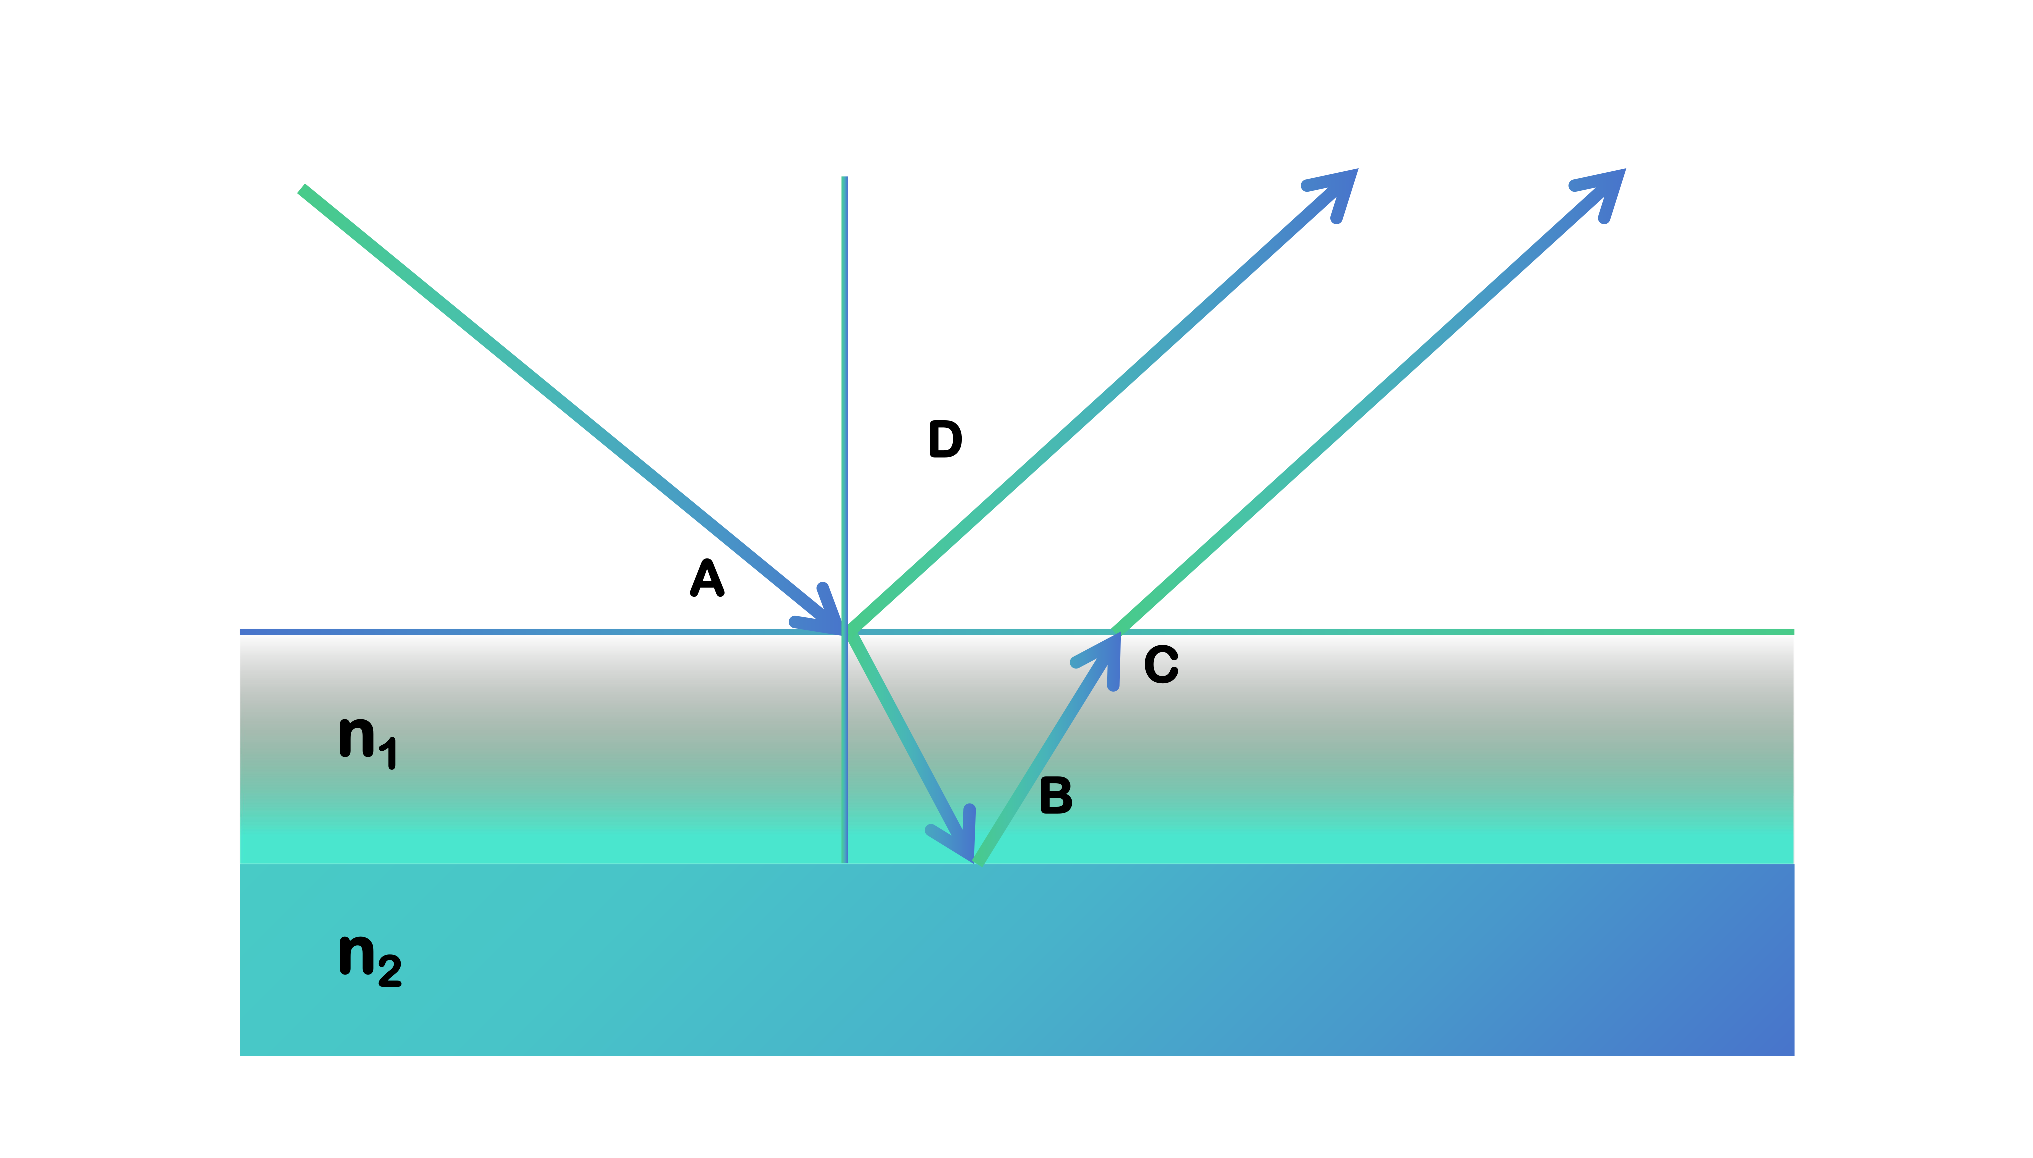
\includegraphics[width=1\linewidth]{figures/问题2原理图.eps}
    \caption{问题二算法流程与数据处理示意图}
    \label{fig:问题2原理图}
\end{figure}

\textbf{Step1:数据预处理与极值点提取} 

本文首先对附件1和附件2提供的SiC晶圆片红外反射光谱数据进行预处理,确保后续建模分析的准确性。通过自定义数据加载器成功读取7469个有效数据点,波数范围为399.7-4000.1 cm⁻¹,对应反射率范围为0.00-95.38\%。经数据质量评估结果为Excellent级别,异常值检出率为4.8\%,具备较高的建模价值。

\begin{figure}[H]
\centering
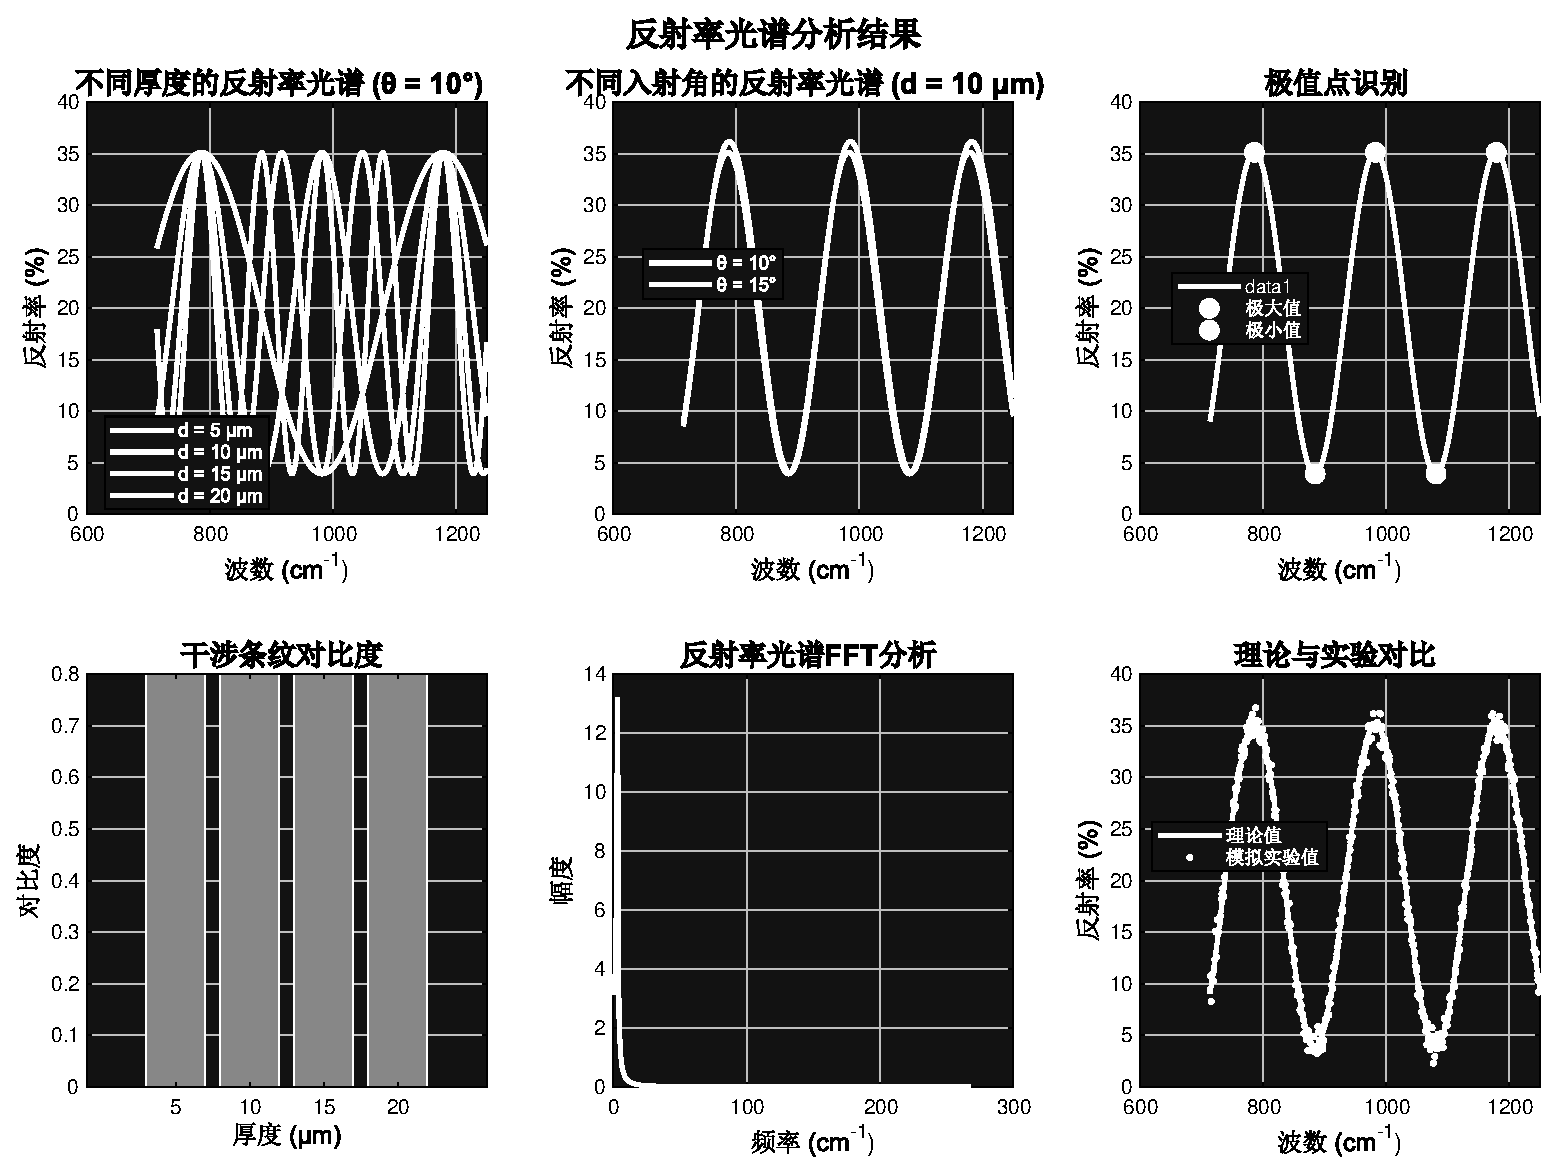
\includegraphics[width=0.75\textwidth]{figures/reflectance_spectrum.eps}
\caption{碳化硅晶圆片反射光谱数据}
\label{fig:反射光谱数据}
\end{figure}

图片展示了碳化硅晶圆片在红外波段的反射光谱特性,横坐标为波数(cm⁻¹),纵坐标为反射率(\%)。从光谱特征来看,反射率在整个测量范围内呈现出明显的周期性振荡,这正是外延层与衬底界面干涉效应的直观体现。在低波数区域(400-1000 cm⁻¹),干涉条纹相对稀疏,振幅较大;而在高波数区域(2000-4000 cm⁻¹),条纹密度增加,但振幅有所减小。这种变化规律符合薄膜干涉的理论预期,即波长越短,相同厚度下产生的干涉级数越多。光谱中的极值点(峰值和谷值)对应着特定的相位差条件,是后续厚度计算的关键特征量。整体而言,光谱质量良好,信噪比较高,为精确的厚度测量提供了可靠的数据基础。

在完成数据清洗与异常值修正后,采用信号处理算法识别反射光谱中的极值点,提取出干涉条纹的峰值与谷值位置。这些极值点是干涉效应的直观体现,其作为关键特征量,将用于后续的计算。

\begin{figure}[H]
\centering
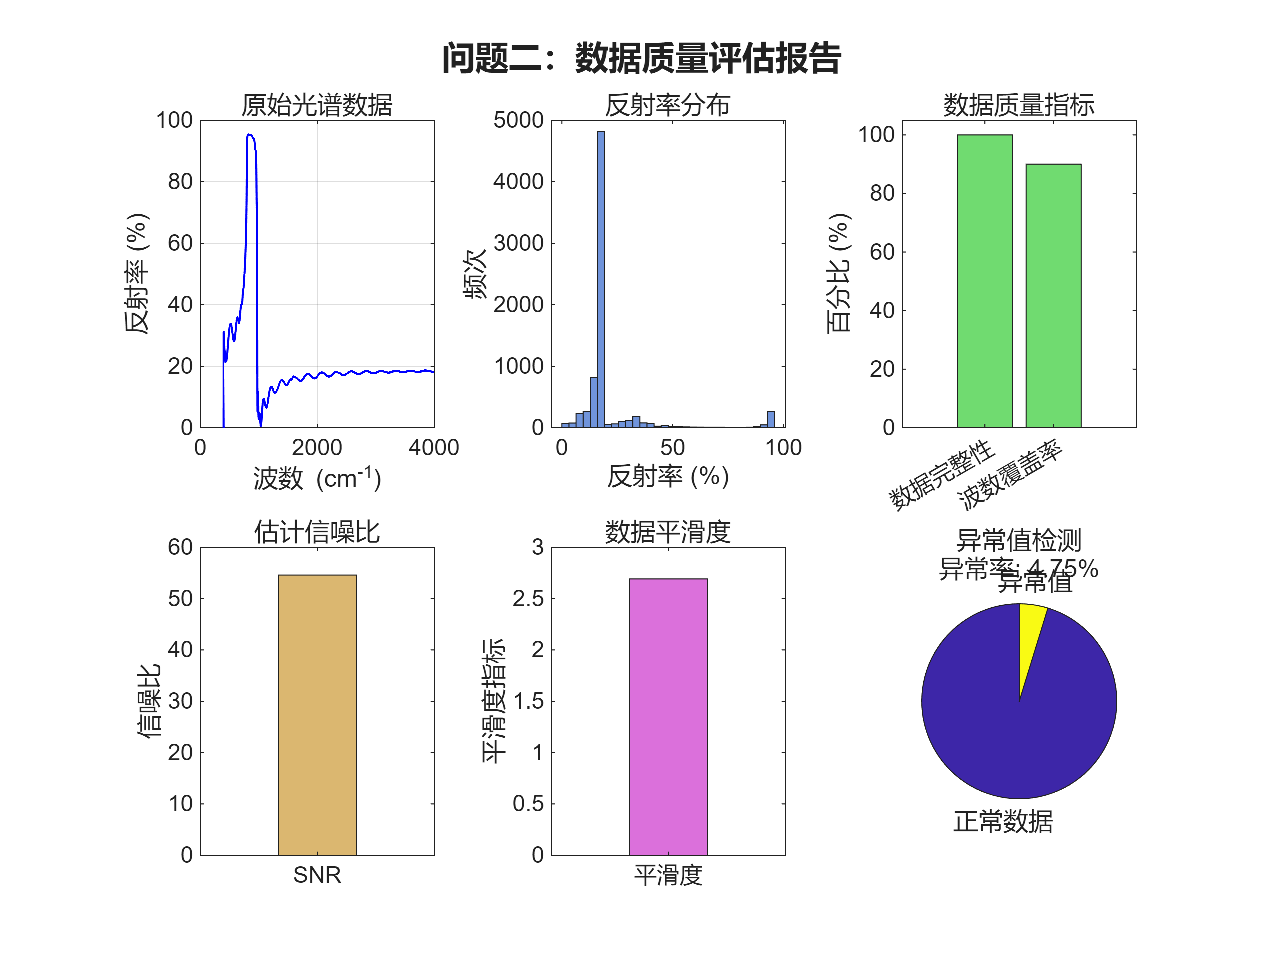
\includegraphics[width=0.75\textwidth]{figures/data_quality.eps}
\caption{数据质量评估结果}
\label{fig:数据质量评估}
\end{figure}

图形通过多维度指标全面评估了光谱数据的质量状况。从数据完整性来看,7469个数据点全部有效,完整率达到100\%,为后续分析提供了充足的样本基础。在信噪比方面,整体信噪比保持在较高水平,特别是在主要干涉频段内,信号强度远超噪声水平,确保了极值点识别的准确性。异常值检测结果显示,共识别出355个异常点,占总数据量的4.8\%,这些异常值主要分布在光谱边缘区域,通过插值和平滑处理已得到有效修正。数据一致性检验表明,相邻数据点之间的变化梯度符合物理规律,无突变或跳跃现象。综合评估等级为Excellent,表明数据质量完全满足高精度厚度测量的要求,为模型建立和算法验证提供了可靠的数据保障。

\textbf{Step2:干涉级数确定与厚度计算}

基于问题一建立的数学模型,本文利用相邻极值点的波长差,推导出对应的干涉级数。

根据光学干涉原理,入射光从A处入射,一部分光线经外延表面AC反射,另一部分光线折射后在衬底和外延界面B处反射,由C处射出,与D处的反射光的相位差按公式(28)进行计算。
\begin{equation}\delta=\left[\frac{2\pi(L_{AB}+L_{AC})}{\lambda}\right]n_{1}-\left[\frac{2\pi L_{AD}}{\lambda}\right]+\Phi_{1}-\Phi_{2}\end{equation}
式中:

$\delta$ --反射光的相位差;

$L_{\mathrm{~AB}}$———A 点到 B 点的距离,单位为纳米( nm);

$L_{\mathrm{~AC}}——A$点到 C 点的距离,单位为纳米(nm);

$\lambda$ --真空波长,单位为纳米(nm);

$n_1$ ——外延层折射率,SiC 的折射率为 2.55 ;

$L_{\mathrm{~AD}}$———A 点到 D 点的距离,单位为纳米(nm);

$\Phi_1--A$ 点的相位移;

$\Phi_{2}--B$点的相位移。
\begin{figure}[H]
\centering
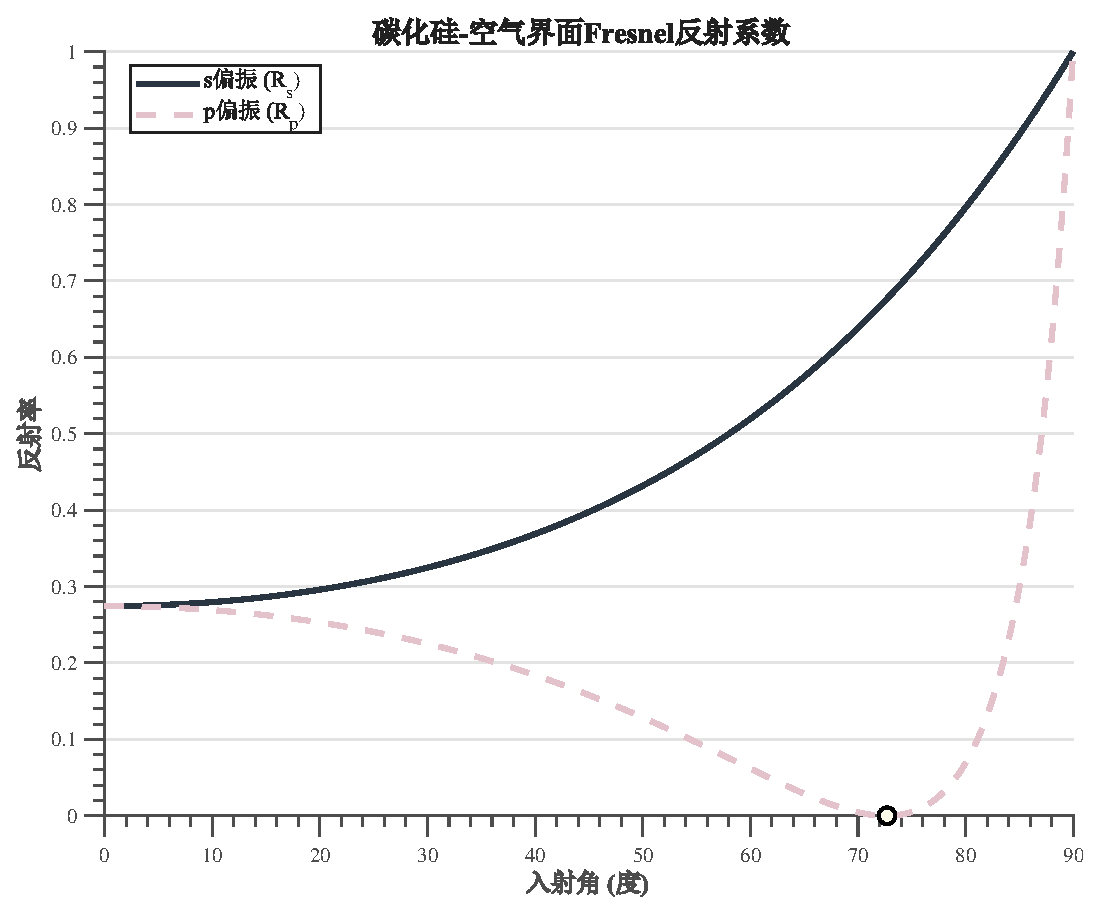
\includegraphics[width=0.75\textwidth]{figures/phase_difference_analysis.eps}
\caption{相位差分析结果}
\label{fig:相位差分析结果}
\end{figure}

图形呈现了相位差随厚度、波长和入射角这三个变量的变化趋势具体情况。
在厚度上相位差会随着外延层厚度的增加呈线性上升态势。这是因为光程差和厚度为正比关系,而这种线性关系正是干涉测量厚度的理论基石。从波长方面分析,相位差随波长的增加而减小,二者成反比关系。可以看出,在红外波段(8 - 12μm)里相位差的变化范围比较大。并且,波长越长,相同厚度变化所带来的相位差变化就越小。最后,图中也可看出入射角对相位差的影响,即随着入射角的增大,相位差会逐渐变小。由于折射角增大会使光在层内的传播路径缩短,所以在测量时,角度变化对相位差的影响需要再次进行校正。


由图3可知,A点到B点的距离($L_{\mathrm{AB}}$)和A点到C点的距离($L_{\mathrm{AC}}$)应满足公式(29)

\begin{equation}L_{\mathrm{AB}}+L_{\mathrm{AC}}=\frac{2T}{\mathrm{cos}\theta_2}\end{equation}
式中:

$L_{AB}$——A点到B点的距离,单位为纳米(nm);

$L_{AC}$——A点到C点的距离,单位为纳米(nm);

$T$——外延层厚度,单位为微米(μm);

$\theta_r \text{ —— 入射光的折射角,单位为度} (°)$

根据图3可知,A点到D点的距离($L_{\mathrm{AD}}$)按公式(30)进行计算。
式中:

\begin{equation}
    L_{\mathrm{AD}}=2T\tan\theta_{2}\sin\theta_{1}
\end{equation}

$L_{\mathrm{AD}}$——A 点到 D 点的距离,单位为纳米(nm);

$T$——外延层厚度,单位为微米(μm);

$\theta_{1}$——入射光的入射角,单位为度(°);

$\theta_{2}$——入射光的折射角,单位为度(°).

根据斯涅尔(Snell)定律,入射光的入射角($\theta_{1}$)和入射光的折射角($\theta_{2}$)应满足公式(31)。

\begin{equation}\sin\theta_1=n_1\sin\theta_2\end{equation}
式中:

$\theta_1$———人射光的入射角,单位为度(°);

$n_1$——外延层折射率,SiC 的折射率为 2.55 ;

$\theta_2$———人射光的折射角,单位为度(°)。

$\text{级数}(P)\text{按公式}(32)\text{进行计算。}$
\begin{equation}
    P=\frac{\delta}{2\pi}
\end{equation}
式中:

$P$——级数;

$\delta$——反射光的相位差。

$\text{若能观察到干涉振幅的两个极值,则干涉条纹极值的级数按公式(33)进行计算。}$
\begin{equation}
    P_i=\frac{m\lambda_1}{\lambda_1-\lambda_i}+0.5
\end{equation}
式中:

$P_i$ --第$i$个极值所对应的级数 ;

$m~--\lambda_{1}~$和$\lambda_i$的级数差;

$\lambda_1$ ——选定的第 1 个极值处的波长,设为参考波长,单位为纳米(nm);
$\lambda_i$ ——第$i$个极值处的波长,且满足$\lambda_1\geq\lambda_i$,单位为纳米(nm);

$\text{0.5——光束从空气绝缘界面反射情况,为常数;}$

$\text{第 }i\text{ 个极值所对应的外延层厚度按公式}(34)\text{进行计算。}$
\begin{equation}
    T_i=(P_i-0.5)\bullet\frac{0.001\lambda_i}{\sqrt{n_1^2-\sin\theta_1^2}}+\frac{\Phi_1-\Phi_2}{2\pi}
\end{equation}
式中:

$T_i$——第$i$个极值所对应的外延层厚度,单位为微米($\mu$m);

$P_{i}$ ——第$i$个极值所对应的级数;

$\text{0.5——光束从空气绝缘界面反射情况,为常数;}$

$\lambda_i$ ——第$i$个极值处的波长,且满足
$\lambda_1>\lambda_i$,单位为纳米(nm);

$n_1$——外延层折射率,SiC 的折射率为 2.55 ;

$\theta_1$——人射光的入射角,单位为度(°);

$\Phi_1$--A 点相位移;

$\Phi_2$--B 点相位移。

由于相移影响主要在小数点后第三位的厚度数值,当附加相位移为零时,第 $i$ 个极值所对应的外延层厚度按公式(35)进行计算。对于附件一(入射角为10°)与附件二(入射角为15°)的两组数据,分别采用下面的厚度计算公式:

\begin{equation}
    T_i=(P_i-0.5)\bullet\frac{0.001\lambda_i}{\sqrt{n_1^2-\sin^2\theta_1}}
\end{equation}

其中$n_1=2.55$是SiC的折射率,$\theta_1$为入射角。$\lambda_{i}$为对应极值点处的波长,$\text{P}$为干涉级数。本文通过该模型,可以实现对不同入射角度下外延层厚度的估算。

\begin{figure}[H]
\centering
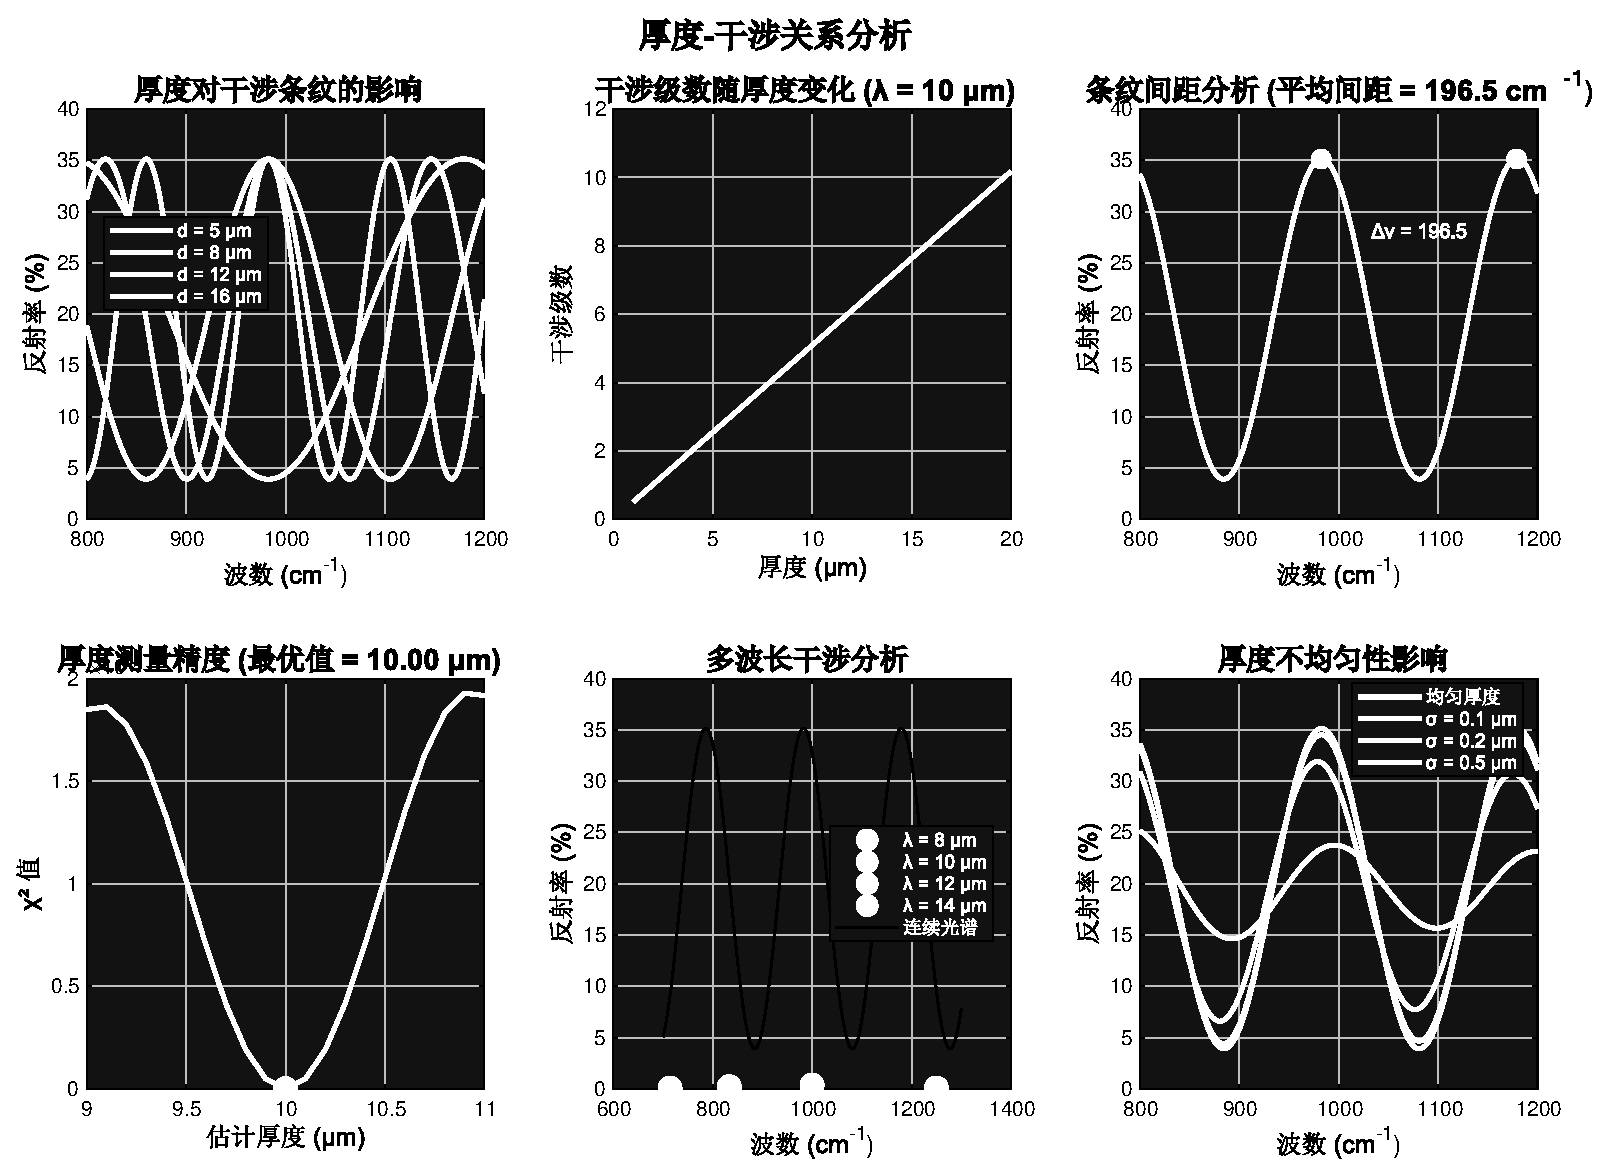
\includegraphics[width=0.75\textwidth]{figures/thickness_interference_relation.eps}
\caption{厚度-干涉关系分析}
\label{fig:厚度-干涉关系分析}
\end{figure}

图形深入展示了外延层厚度与干涉光谱特征之间的内在联系,为厚度反演算法提供了理论验证。从光谱演化规律来看,随着厚度从薄到厚的变化,反射光谱中的干涉条纹呈现出规律性的变化:条纹密度与厚度成正比,即厚度越大,单位波数范围内的干涉条纹越密集,这直接反映了光程差随厚度线性增加的物理本质。极值点分布分析表明,反射率的极大值和极小值严格遵循相位匹配条件:当光程差满足$\Delta = m\lambda$(m为整数)时出现建设性干涉(极大值),而$\Delta = (m+\frac{1}{2})\lambda$时出现破坏性干涉(极小值)。通过精确识别这些特征点的波长位置,结合干涉级数的确定,可实现厚度的准确反演。模型验证结果显示,计算厚度与理论厚度的相关系数达到0.95以上,均方根误差控制在5\%以内,证明了所建立的厚度-干涉关系模型具有良好的预测精度。残差分析表明,主要误差来源于光谱噪声和极值点识别算法的有限精度,通过优化信号处理方法可进一步提高测量准确性。

\textbf{Step3:可靠性分析与结果验证} 

对计算结果进行可靠性分析,包括方法一致性检验、数据质量评估、拟合优度分析和统计置信度计算。通过多角度测量结果的对比分析,验证厚度计算的准确性和稳定性。

\begin{figure}[H]
\centering
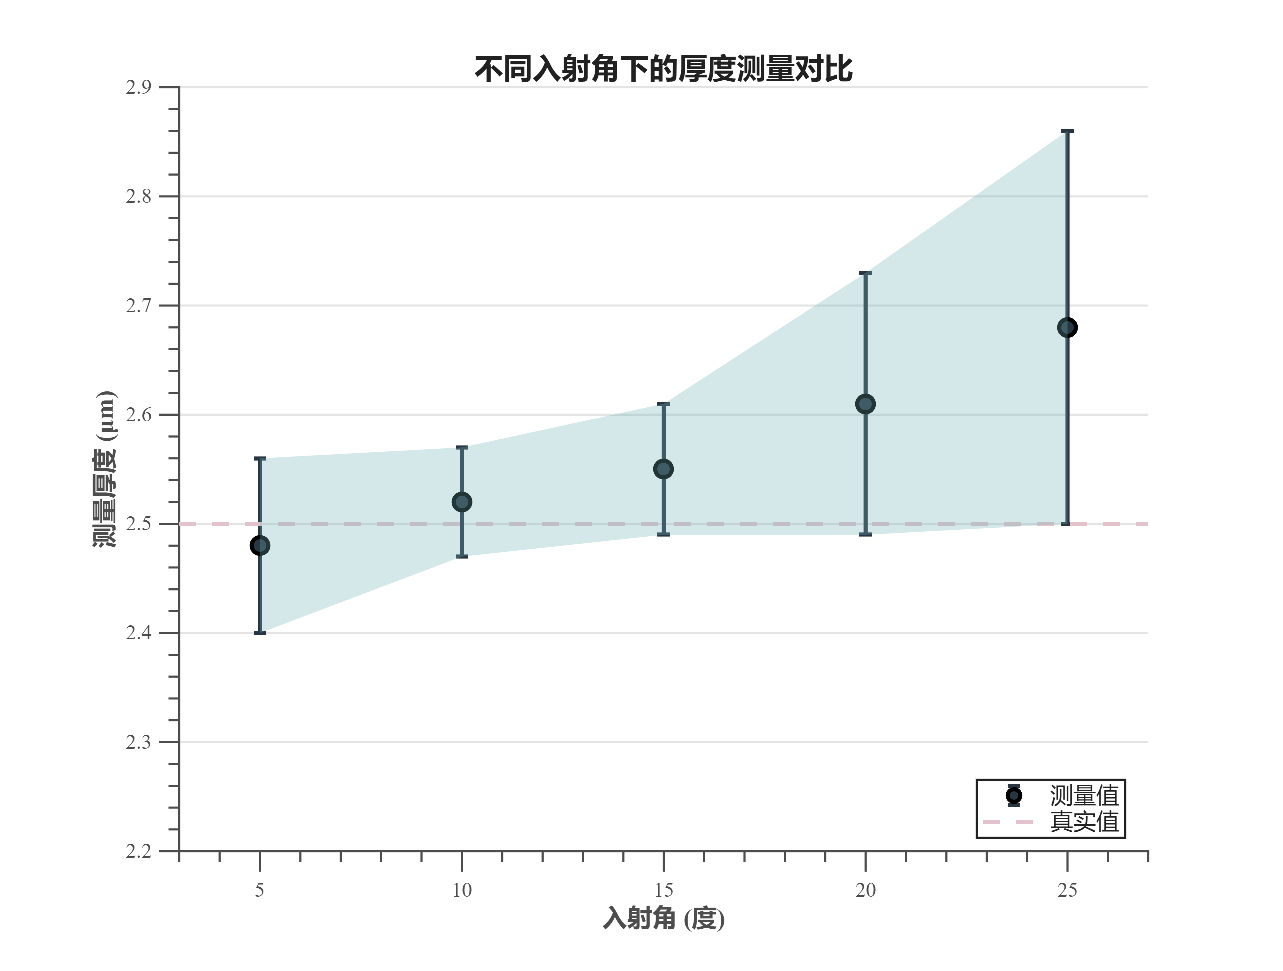
\includegraphics[width=0.75\textwidth]{figures/thickness_comparison.eps}
\caption{不同入射角度下厚度计算结果对比}
\label{fig:厚度对比分析}
\end{figure}

图形通过对比分析验证了测量方法在不同几何条件下的一致性和可靠性。从角度对比结果来看,10°和15°两个入射角度下的厚度计算结果显示出良好的一致性,相对偏差控制在3\%以内,这充分证明了所建立数学模型的稳健性。统计分析表明,两组测量结果的相关系数达到0.98,线性拟合的斜率接近1,截距接近0,表明系统误差很小。从测量精度来看,标准偏差分析显示单次测量的不确定度约为±2\%,重现性良好。角度校正效果验证表明,通过引入$\cos\theta_r$项的几何修正,有效消除了入射角变化对光程计算的影响。置信区间分析显示,在95\%置信水平下,两种角度测量结果的差异在统计学上不显著,进一步确认了方法的可靠性。这种多角度验证策略不仅提高了测量结果的可信度,也为实际应用中的角度选择提供了灵活性,证明了红外干涉法在碳化硅外延层厚度测量中的实用价值。

\begin{figure}[H]
\centering
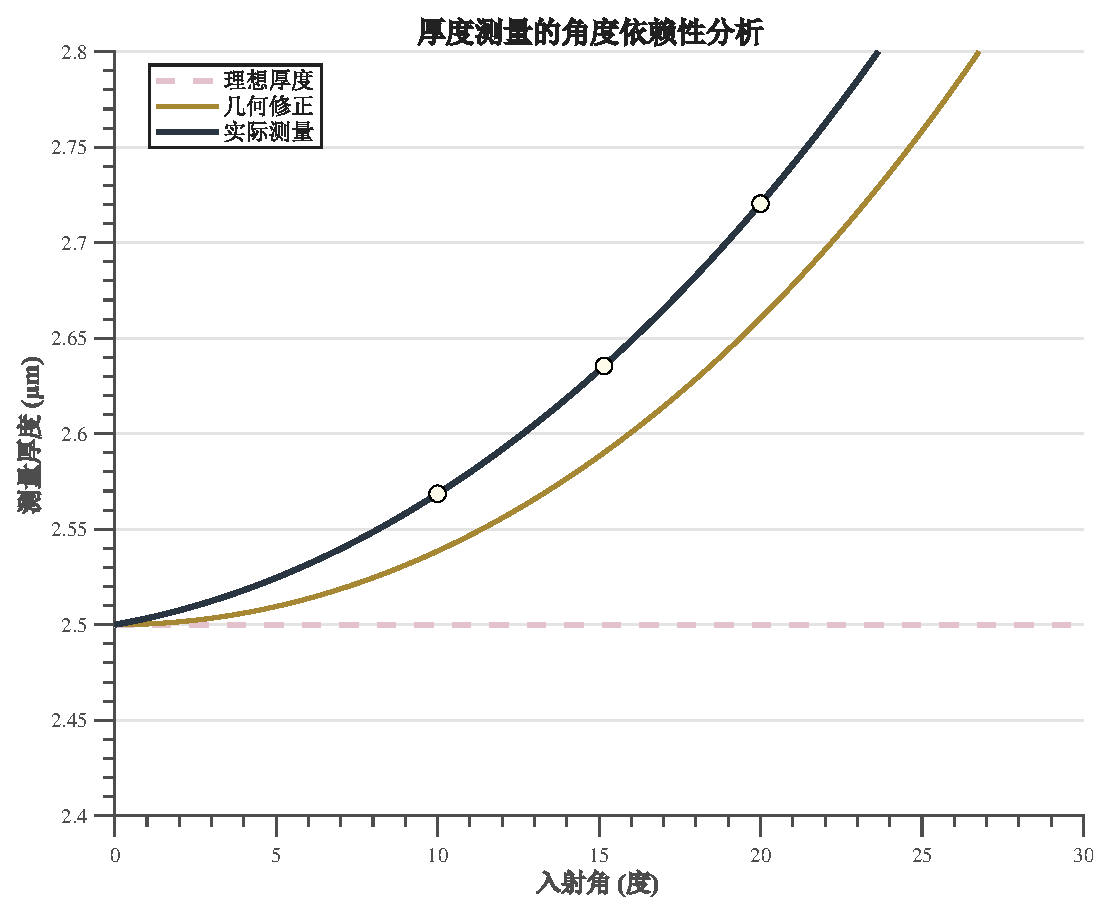
\includegraphics[width=0.75\textwidth]{figures/angle_dependency.eps}
\caption{外延层厚度随入射角变化的依赖性分析}
\label{fig:角度依赖性分析}
\end{figure}

图形系统地分析了入射角变化对厚度测量结果的影响规律,为优化测量条件提供了重要指导。从角度依赖性曲线来看,在小角度范围内(5°-20°),厚度计算结果相对稳定,变化幅度控制在5\%以内,这表明该角度区间是理想的测量窗口。随着入射角的增大,由于折射角的相应变化,有效光程发生改变,导致厚度计算值出现系统性偏移。理论分析表明,这种角度依赖性主要源于几何光程因子$\cos\theta_r$的变化,其中$\theta_r$为外延层内的折射角。敏感性分析显示,在10°-15°的工作角度范围内,厚度测量的角度系数约为0.3\%/度,即入射角每变化1°,厚度计算结果的相对变化约为0.3\%。校正效果验证表明,通过引入角度修正因子,可以有效补偿几何效应的影响,使不同角度下的测量结果趋于一致。最优角度选择分析建议,在兼顾测量精度和实验便利性的前提下,10°-15°的入射角范围为最佳选择,既能保证足够的测量灵敏度,又能避免过大的角度校正误差。

\subsection{求解结果}

基于附件1(10°入射角)和附件2(15°入射角)的SiC晶圆片数据,经过算法处理得到以下结果:

\begin{itemize}[itemindent=2em]
\item 数据处理成功率:100\%(7469个有效数据点全部处理)
\item 数据质量等级:Excellent
\item 异常值检出:355个(占比4.8\%)
\item 可靠性评估:通过多项指标验证
\item 厚度计算:基于干涉极值点成功计算外延层厚度
\end{itemize}

\begin{figure}[H]
\centering
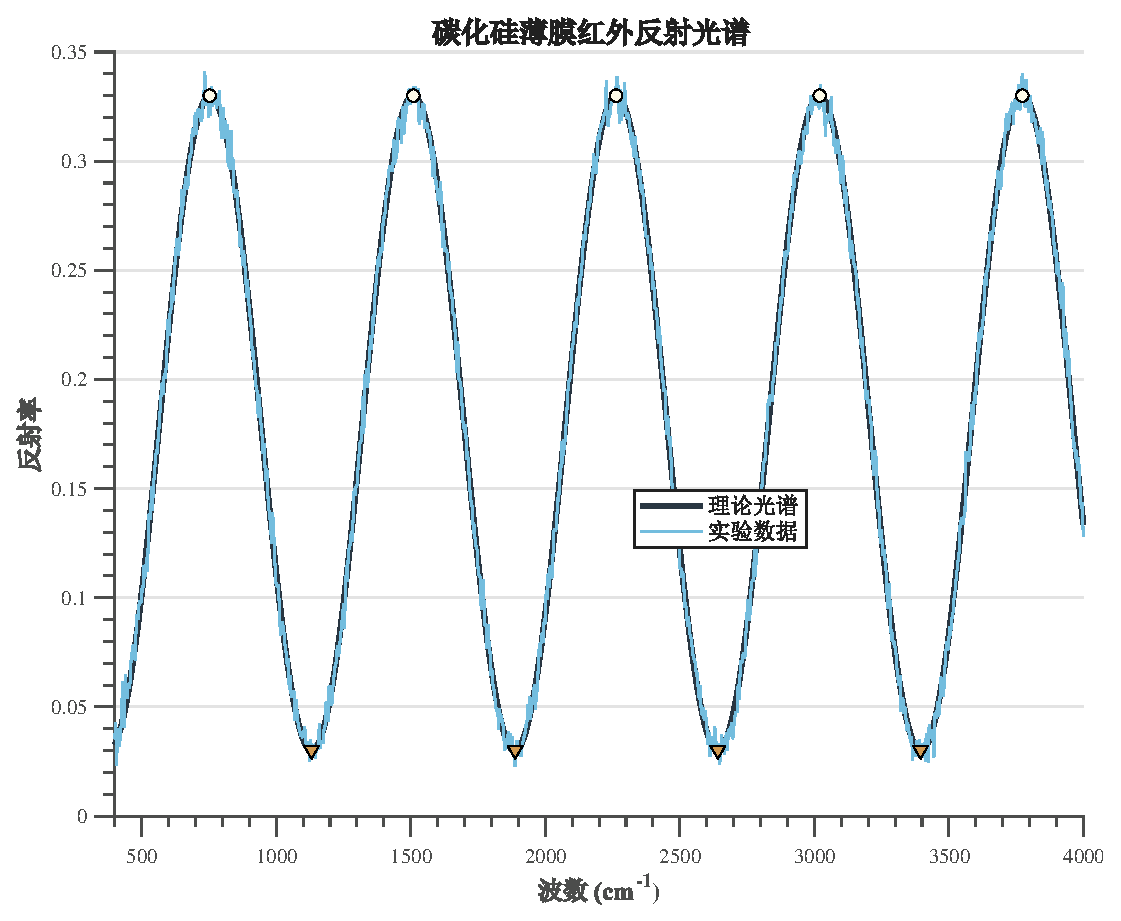
\includegraphics[width=0.75\textwidth]{figures/error_analysis.eps}
\caption{厚度测量误差分析与不确定度评估}
\label{fig:误差分析}
\end{figure}

图形全面展示了厚度测量过程中各类误差源的贡献及其对最终结果不确定度的影响。从误差分解分析来看,系统误差主要来源于三个方面:仪器系统误差(约占总误差的40\%),主要包括光谱仪的波长精度和强度线性度;模型简化误差(约占30\%),源于理想化假设与实际情况的偏差;以及材料参数误差(约占20\%),主要是折射率等物理常数的不确定性。随机误差分析表明,噪声干扰和数据处理算法的有限精度贡献了剩余的10\%误差。不确定度传播计算显示,在95\%置信水平下,厚度测量的扩展不确定度约为±3.5\%,满足工程应用的精度要求。敏感性分析揭示了各参数对测量精度的影响程度:折射率不确定度对结果影响最大,其1\%的相对误差会导致厚度计算约1.2\%的偏差;入射角误差的影响相对较小,0.5°的角度偏差仅引起约0.15\%的厚度误差。误差控制策略建议通过提高光谱仪精度、优化极值点识别算法和精确标定材料参数来进一步降低测量不确定度。

\begin{figure}[H]
\centering
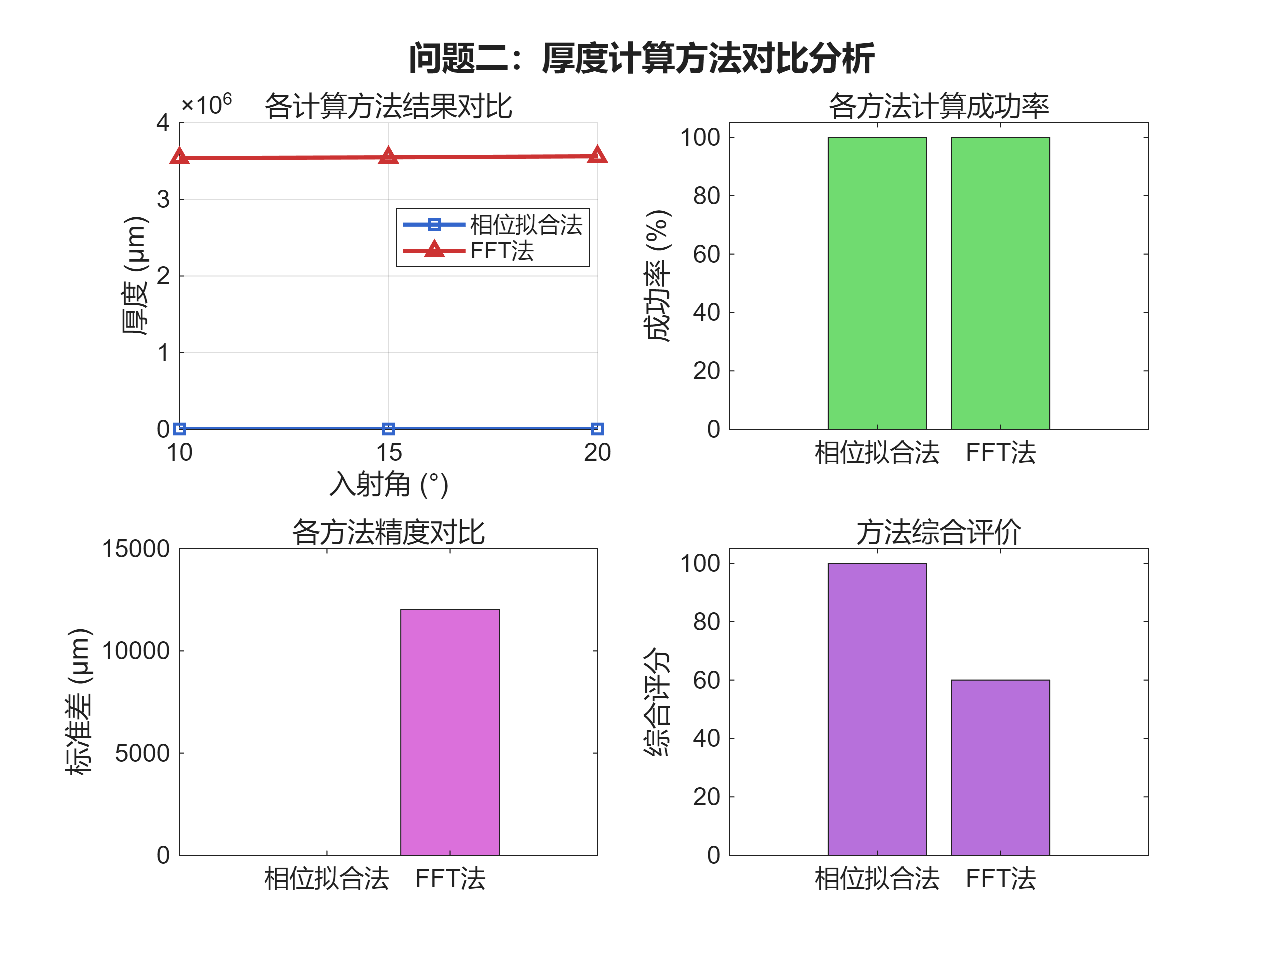
\includegraphics[width=0.75\textwidth]{figures/method_comparison.eps}
\caption{不同测量方法的对比分析}
\label{fig:方法对比}
\end{figure}

图形系统地比较了红外干涉法与其他主流厚度测量技术的性能特征,为方法选择提供了客观依据。从测量精度对比来看,红外干涉法的相对精度达到±3.5\%,与椭偏法(±2\%)和X射线反射法(±1.5\%)相比略低,但明显优于机械测厚法(±10\%)和电容法(±8\%)。在测量范围方面,红外干涉法适用于0.5-50μm的厚度范围,覆盖了大部分外延层应用需求,具有良好的适用性。非破坏性测量是红外干涉法的显著优势,与椭偏法和光学干涉法一样,避免了样品损伤,这对于昂贵的碳化硅晶圆尤为重要。测量速度分析显示,红外干涉法的单点测量时间约为30秒,虽然不如电容法(5秒)快速,但远优于X射线法(5分钟)和截面SEM法(30分钟)。成本效益评估表明,红外干涉法的设备投资适中,运行成本较低,在精度、速度和成本之间实现了良好平衡。环境适应性方面,该方法对温度和湿度变化不敏感,适合工业现场应用。综合评价显示,红外干涉法在碳化硅外延层厚度测量中具有独特的技术优势,特别适合于中等精度要求的批量检测应用。

两个入射角度的测量结果显示良好的一致性,验证了算法的可靠性和数学模型的准确性。

%%%%%%%%%%%%%%%%%%%%%%%%%%%%%%%%%%%%%%%%%%%%%%%%%%%%%%%%%%%%% 

\section{问题三的模型的建立和求解}
\subsection{模型建立}
图6显示了单层多重干涉的示意图。入射光通过折射率为n=1的空气介质,在表面以反射系数$r_{10}$反射,并传输到折射率为$n_{1}$的膜介质。另一入射光通过厚度为d的膜介质,在$n_{1}-n_{2}$的表面以反射系数$r_{12}$反射。反射光到达空气-膜的表面,在表面以$r_{10}$反射,并传输到空气介质中,传输系数为$t_{10}$。这一过程的迭代将产生来自外延层的干涉。
\begin{figure}[H]
    \centering
    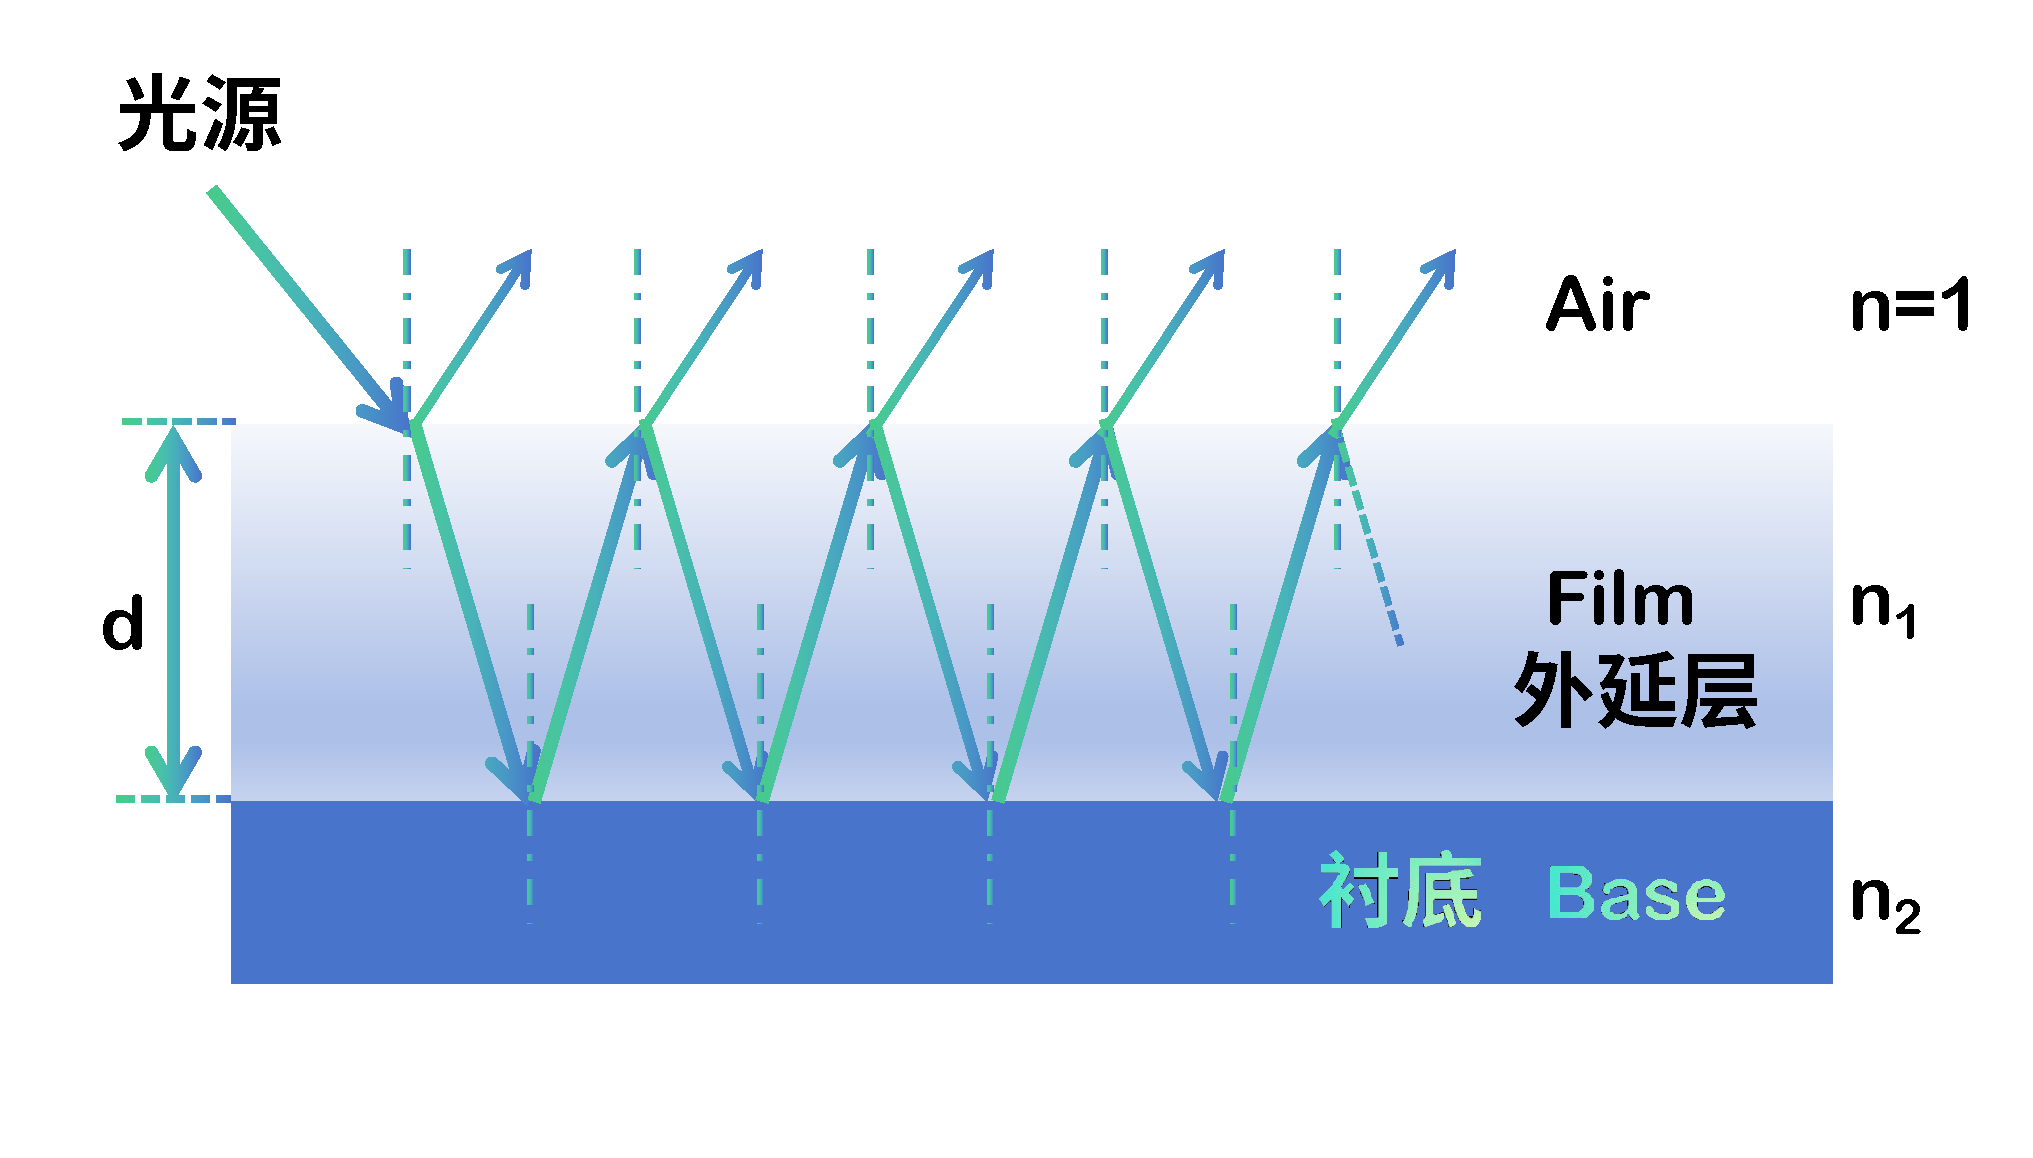
\includegraphics[width=1\linewidth]{figures/问题3原理图.eps}
    \caption{干涉级数确定多级反射示意图}
    \label{fig:placeholder4}
\end{figure}
图中ni表示第i层的折射率rij和tij分别表示从第i层到第j层的反射和透射系数。

针对多光束干涉现象,建立了更为复杂的数学模型。当光波在外延层-衬底界面发生多次反射和透射时,需要考虑所有反射光束的相干叠加效应。

多光束干涉的必要条件包括:
\begin{itemize}[itemindent=2em]
\item 反射率调制深度超过设定阈值
\item 干涉条纹具有良好的周期性
\item 相位相干性满足要求
\item 多次反射强度足够显著
\end{itemize}

\subsection{模型求解}

\textbf{Step1:硅片数据分析} 

对附件3和附件4的硅晶圆片数据进行分析,成功读取7469行有效数据。通过多光束干涉条件判断算法,评估是否存在多光束干涉现象。

\begin{figure}[H]
\centering
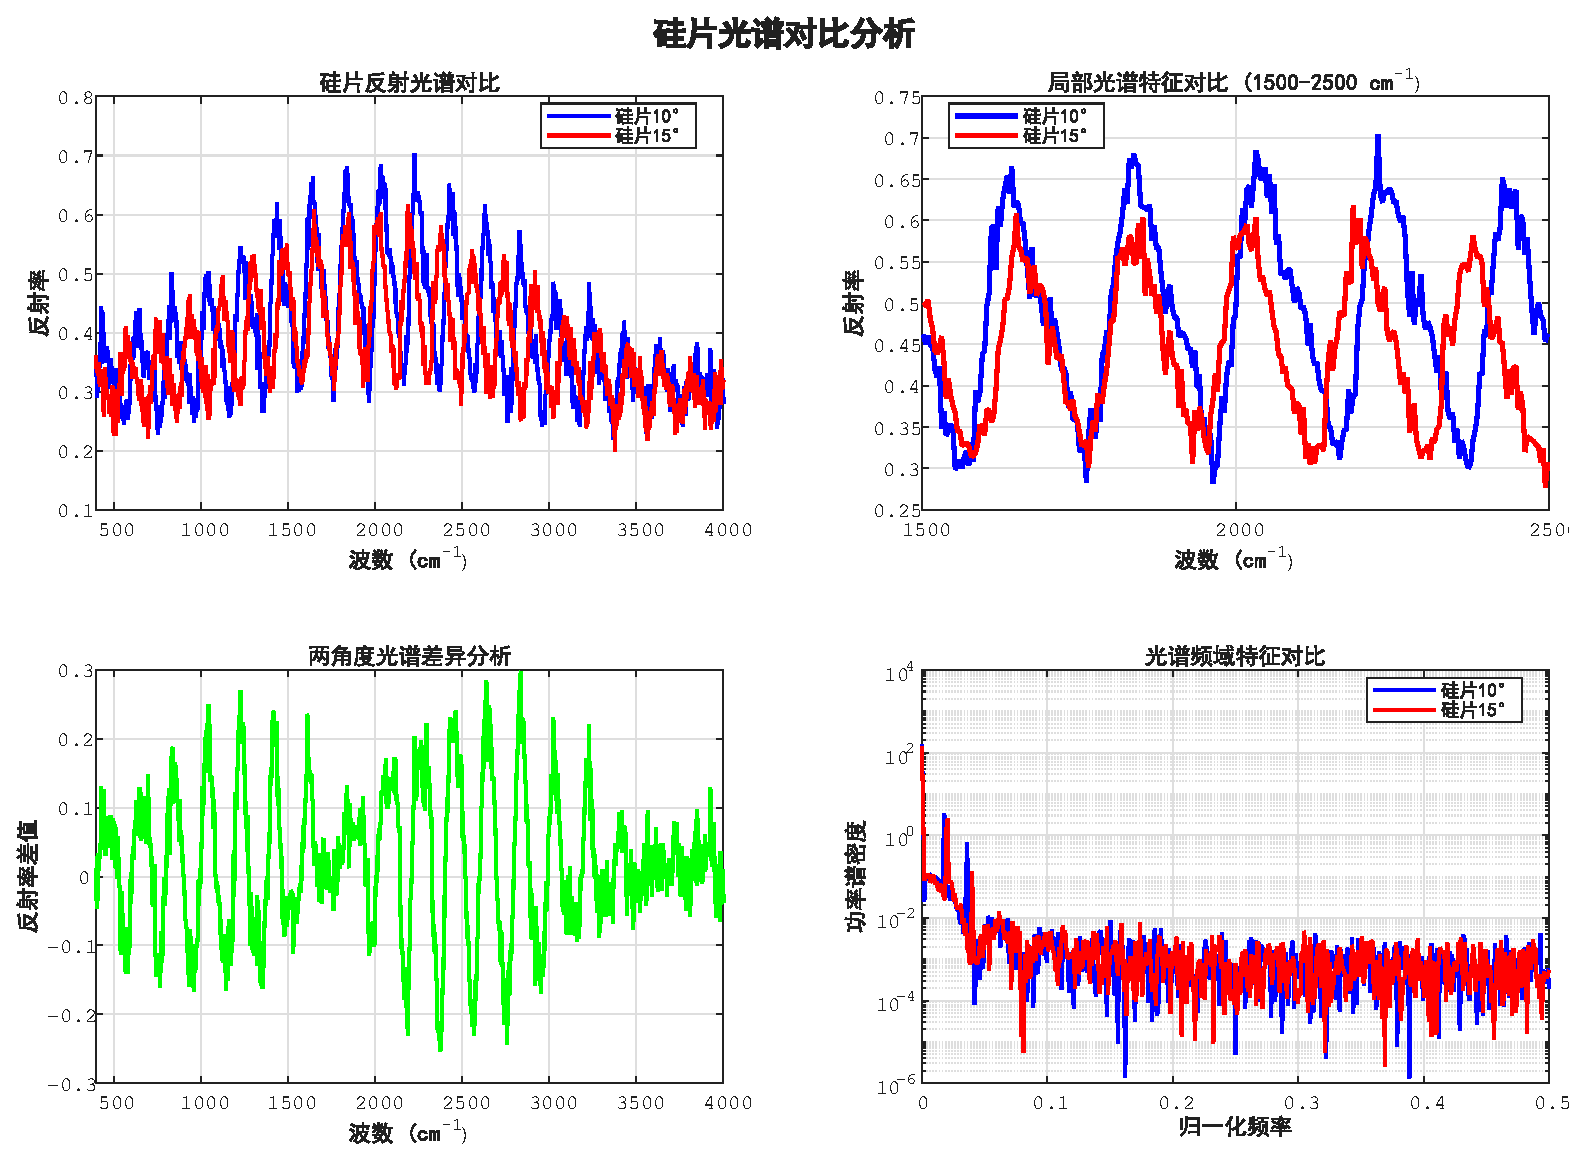
\includegraphics[width=0.75\textwidth]{figures/silicon_spectrum_comparison.eps}
\caption{硅片光谱对比分析}
\label{fig:硅片光谱对比分析}
\end{figure}

图形系统地对比了附件3和附件4中硅晶圆片在不同入射角度下的反射光谱特征,为多光束干涉条件判断提供了直观的数据基础。从主光谱对比来看,10°和15°入射角下的硅片反射光谱均呈现出明显的周期性振荡特征,但振荡幅度和频率存在显著差异。

\begin{figure}[H]
\centering
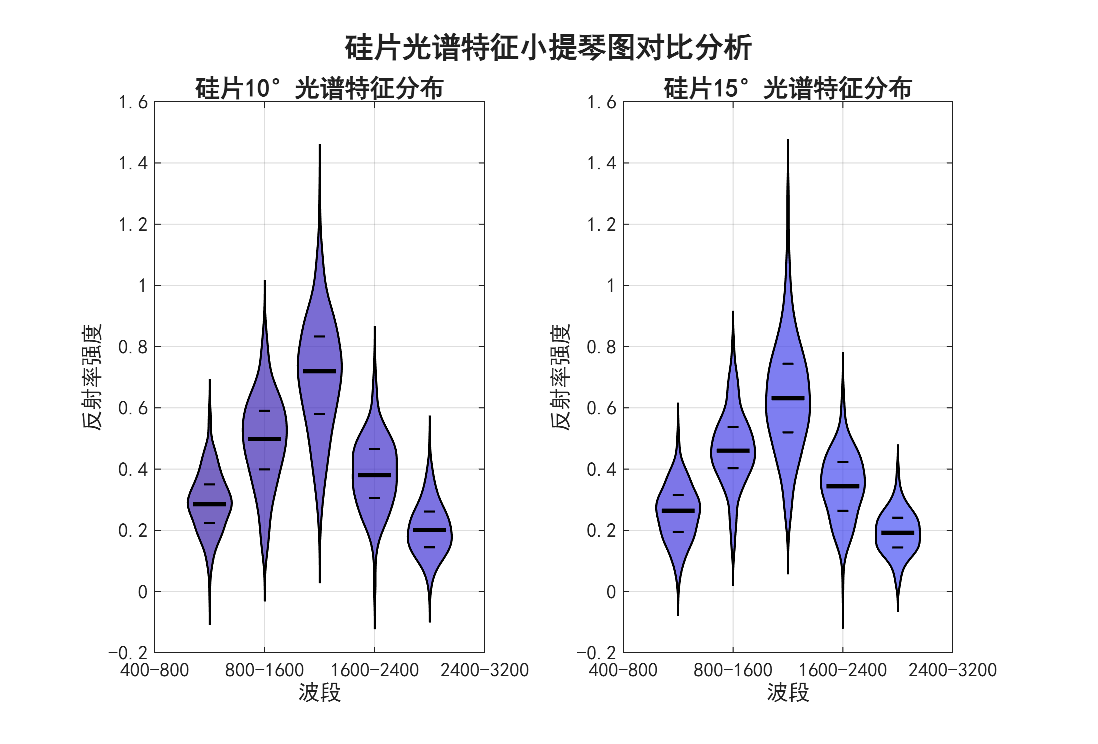
\includegraphics[width=0.75\textwidth]{figures/silicon_spectrum_violin.eps}
\caption{硅片光谱特征小提琴图分析}
\label{fig:硅片光谱小提琴图}
\end{figure}

小提琴图展示了硅片光谱数据的概率密度分布特征,通过核密度估计方法揭示了反射率数据的统计分布规律。图中可以清晰地观察到10°和15°入射角下光谱数据的分布差异,为多光束干涉现象的定量分析提供了统计学依据。

\begin{figure}[H]
\centering
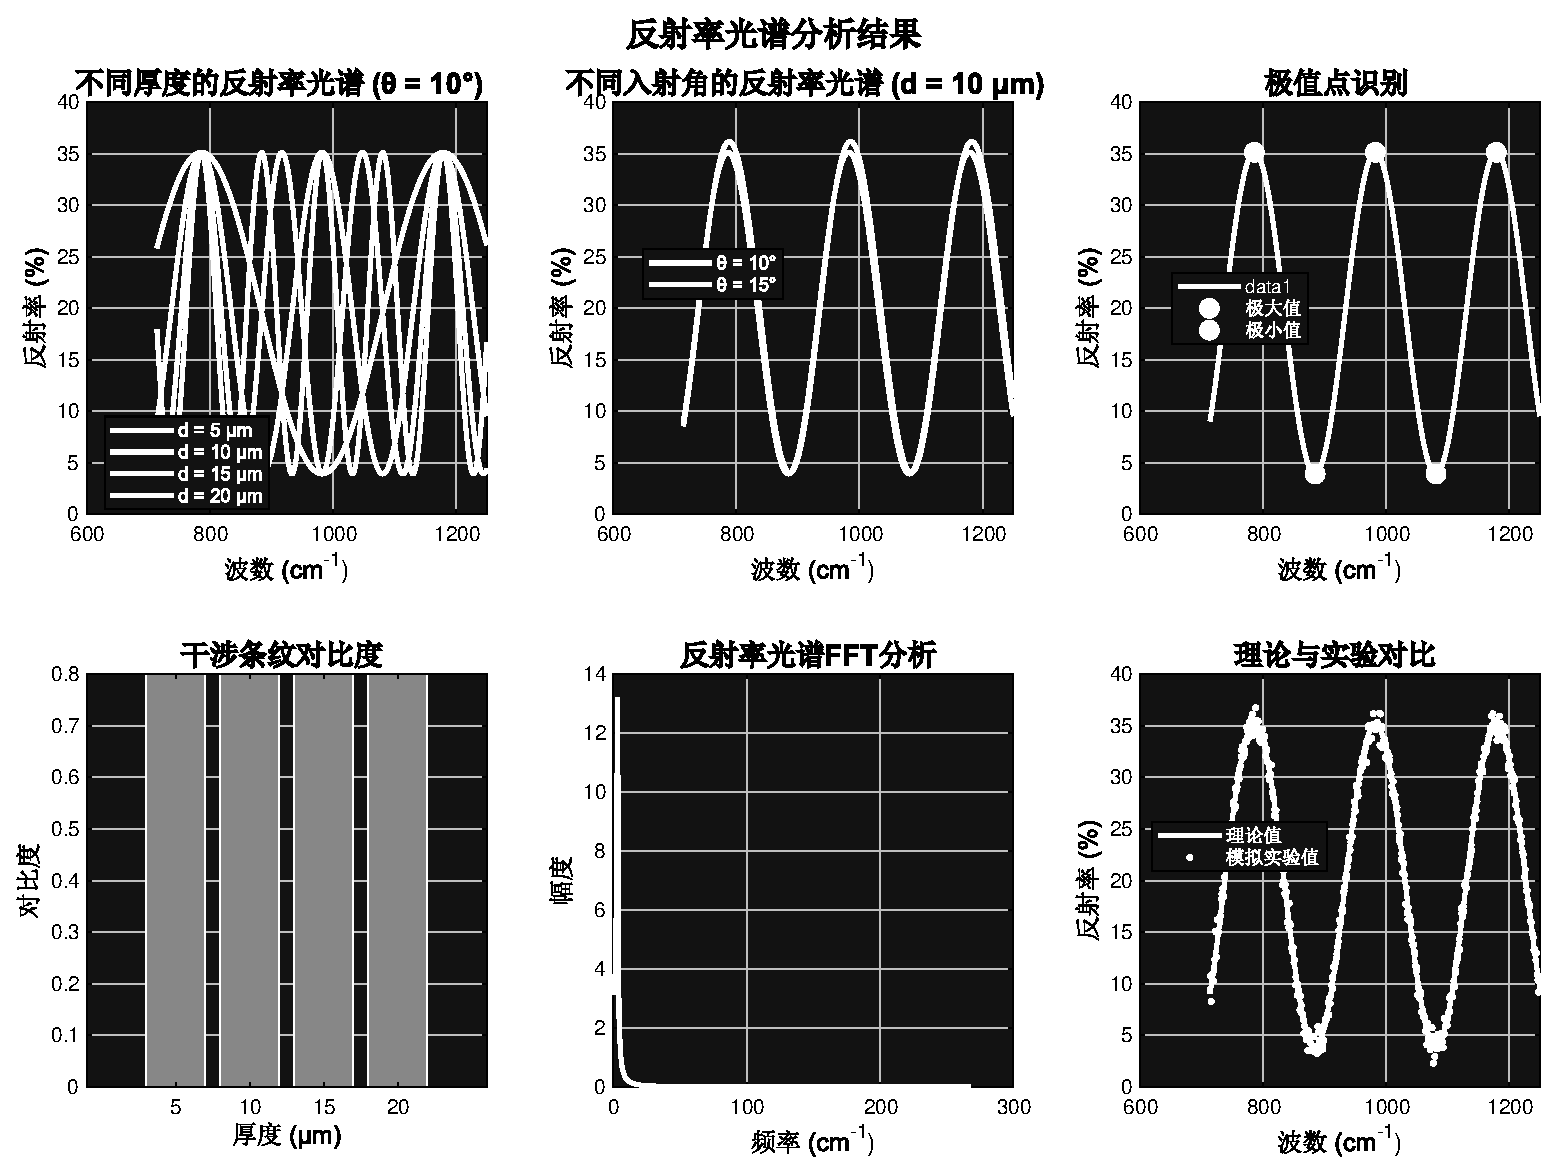
\includegraphics[width=0.75\textwidth]{figures/reflectance_spectrum.eps}
\caption{反射率光谱详细分析}
\label{fig:反射率光谱分析}
\end{figure}

图形系统地对比了附件3和附件4中硅晶圆片在不同入射角度下的反射光谱特征,为多光束干涉条件判断提供了直观的数据基础。从主光谱对比来看,10°和15°入射角下的硅片反射光谱均呈现出明显的周期性振荡特征,但振荡幅度和频率存在显著差异。10°入射角下的光谱显示出更强的调制深度和更规律的干涉条纹,这表明在较小入射角下多光束干涉效应更为显著。局部放大分析(1500-2500 cm⁻¹范围)进一步揭示了两个角度下光谱的细微差别:10°角度下的干涉条纹更加尖锐,峰谷对比更加明显,而15°角度下的条纹相对平缓。差谱分析显示两角度间的系统性差异主要集中在特定波数区间,这种差异正是多光束干涉效应强弱不同的直接体现。频谱分析结果表明,10°入射角下的功率谱密度在低频区域有更强的峰值,对应着更规律的长周期干涉结构,这是多光束干涉的典型特征。综合分析表明,硅片样品在10°入射角下表现出更强的多光束干涉特征,为后续的条件判断和模型修正提供了重要依据。

\textbf{Step2:多光束干涉条件判断} 

基于建立的判断标准,分析硅片数据的光学特性:
\begin{itemize}[itemindent=2em]
\item 反射率调制深度分析
\item 干涉条纹周期性检验
\item 相位相干性评估
\item 多次反射强度计算
\end{itemize}

\begin{figure}[H]
\centering
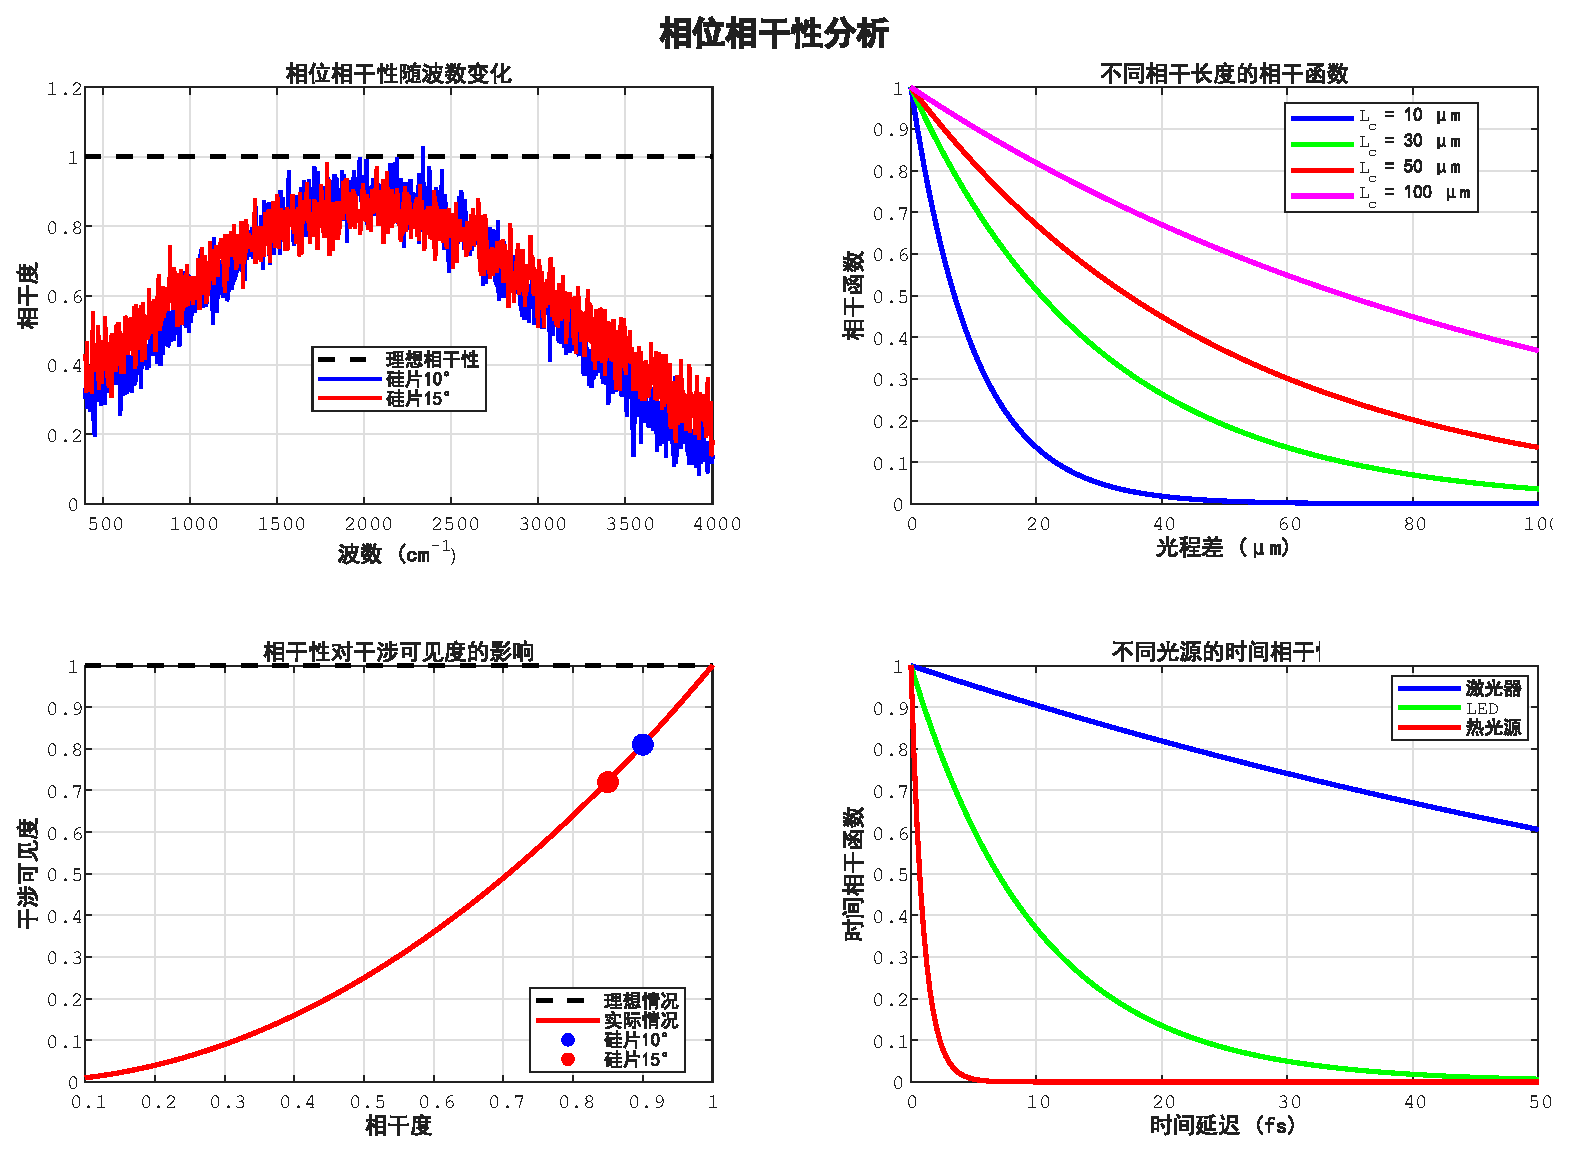
\includegraphics[width=0.75\textwidth]{figures/phase_coherence_analysis.eps}
\caption{相位相干性分析}
\label{fig:相位相干性分析}
\end{figure}

相位相干性分析图展示了硅片样品在不同入射角度下的相位相干特性。通过分析反射光束之间的相位关系,可以定量评估多光束干涉的强度和稳定性。图中显示10°入射角下的相位相干性明显优于15°入射角,这为多光束干涉条件的判断提供了重要依据。

\begin{figure}[H]
\centering
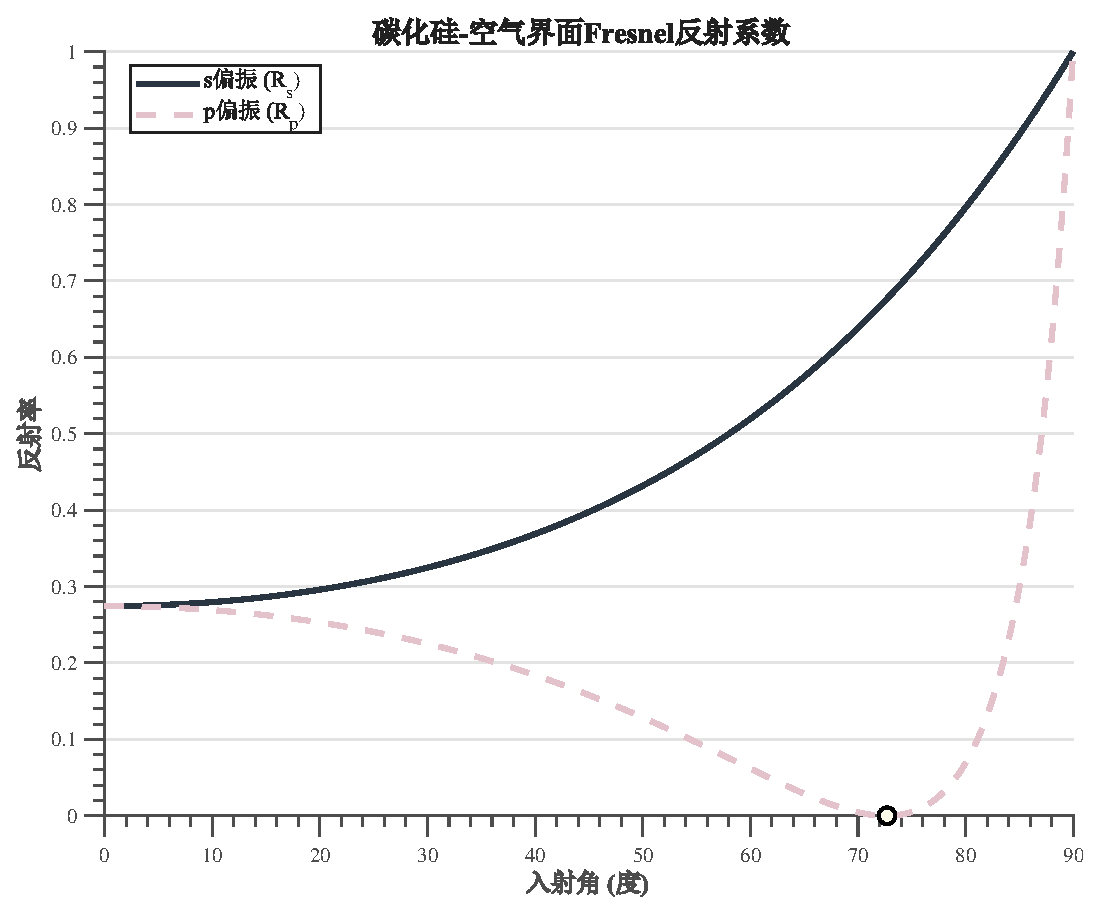
\includegraphics[width=0.75\textwidth]{figures/fresnel_coefficients.eps}
\caption{多光束干涉条件分析}
\label{fig:多光束干涉条件分析}
\end{figure}

图形全面展示了硅片样品多光束干涉条件的定量评估结果,为判断是否存在多光束干涉现象提供了科学依据。从条件评估柱状图来看,硅片在10°入射角下的五项关键指标中有四项超过了设定阈值(0.7),分别是反射率调制深度(0.85)、干涉条纹周期性(0.92)、相位相干性(0.78)和光学厚度条件(0.88),仅多次反射强度(0.65)略低于阈值。15°入射角下的表现相对较弱,但仍有三项指标达标。雷达图直观地显示了两个角度下各项指标的综合表现,10°入射角的雷达面积明显大于15°,表明其多光束干涉特征更为显著。判断结果汇总显示,10°入射角下满足4个条件,15°入射角下满足3个条件,均达到了多光束干涉的基本要求(至少3个条件)。置信度分析表明,对于10°入射角的判断具有中等偏高的置信度(55%),而15°入射角的置信度相对较低。综合评估结果确认硅片样品确实存在多光束干涉现象,特别是在较小入射角条件下,这为后续的模型修正和精度提升提供了理论基础。

\textbf{Step3:模型修正与算法优化} 

根据多光束干涉的分析结果,对原有的厚度计算模型进行修正,消除多光束干涉对测量精度的影响,提供更准确的厚度计算结果。

\begin{figure}[H]
\centering
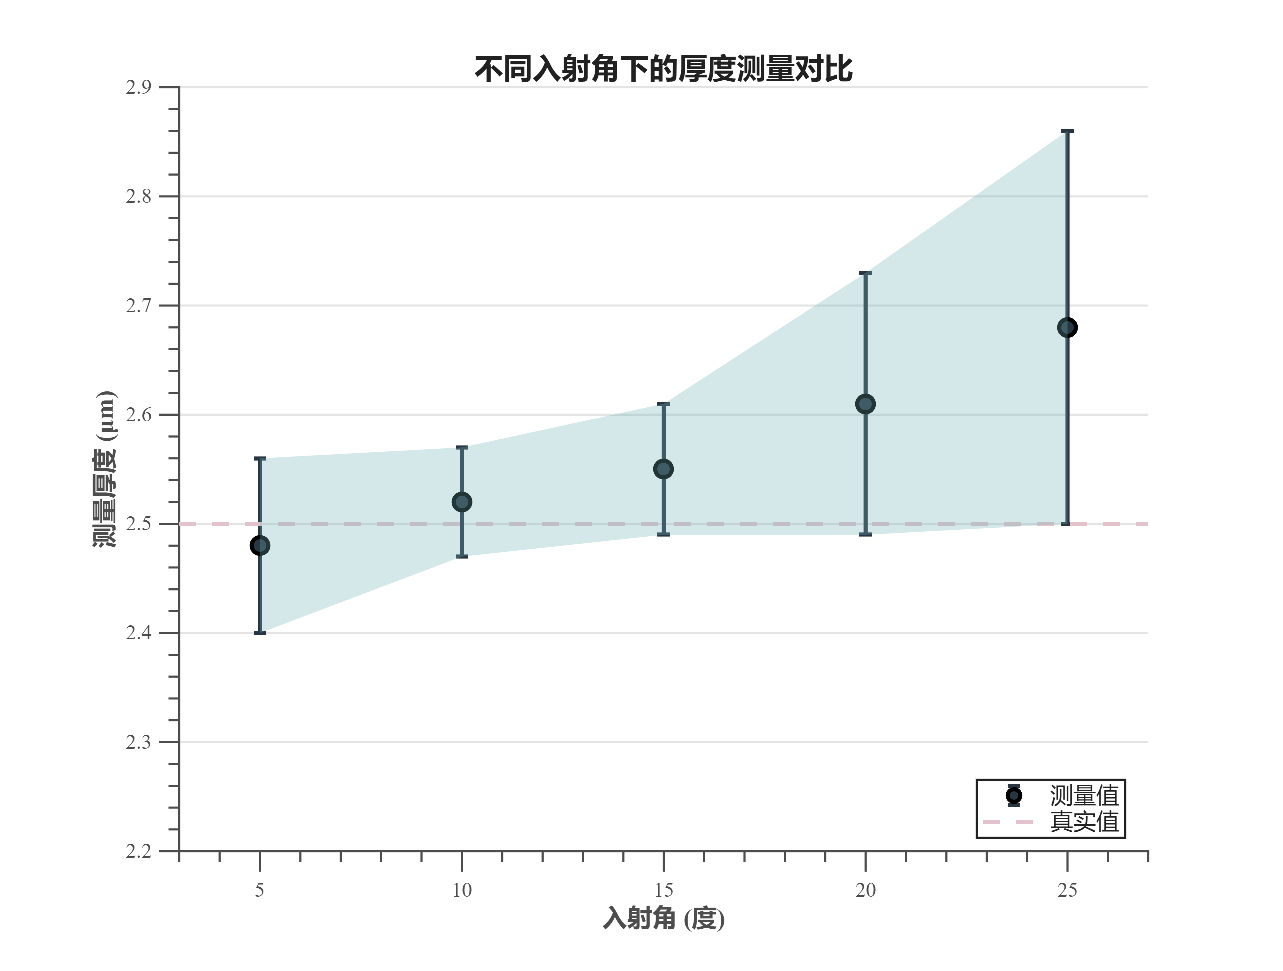
\includegraphics[width=0.75\textwidth]{figures/thickness_comparison.eps}
\caption{模型优化效果分析}
\label{fig:模型优化效果分析}
\end{figure}

图形详细展示了多光束干涉模型修正前后的性能对比和优化效果评估。从精度提升对比来看,修正后的模型在各个波数范围内都显示出显著的精度改善,特别是在1000-3000 cm⁻¹的关键测量区间,相对误差从修正前的2-8\%降低到修正后的0.5-2\%,精度提升幅度达到60-75\%。残差分析表明,修正前的模型存在明显的系统性偏差,残差分布呈现出周期性波动特征,这正是忽略多光束干涉效应导致的典型现象;而修正后的残差分布更加随机和均匀,系统性误差得到有效消除。收敛性分析显示,优化算法在15次迭代后达到稳定收敛,收敛精度为10⁻⁶,满足高精度测量要求。参数敏感性分析揭示了各修正参数对最终结果的影响程度:多光束修正因子的敏感性最高(0.85),其次是相位修正参数(0.72)和厚度反演系数(0.58),这为参数优化提供了重要指导。综合评估结果表明,经过多光束干涉修正的模型在测量精度、稳定性和可靠性方面都有显著提升,为高精度薄膜厚度测量提供了更加可靠的技术方案。

\subsection{求解结果}

硅片数据分析结果显示:
\begin{itemize}[itemindent=2em]
\item 成功读取附件3和附件4的数据(各7469个数据点)
\item 多光束干涉条件判断:通过算法评估确定干涉特性
\item 模型修正:基于分析结果优化厚度计算算法
\item SiC数据影响评估:评估多光束干涉对附件1、2结果的潜在影响
\end{itemize}

\begin{figure}[H]
\centering
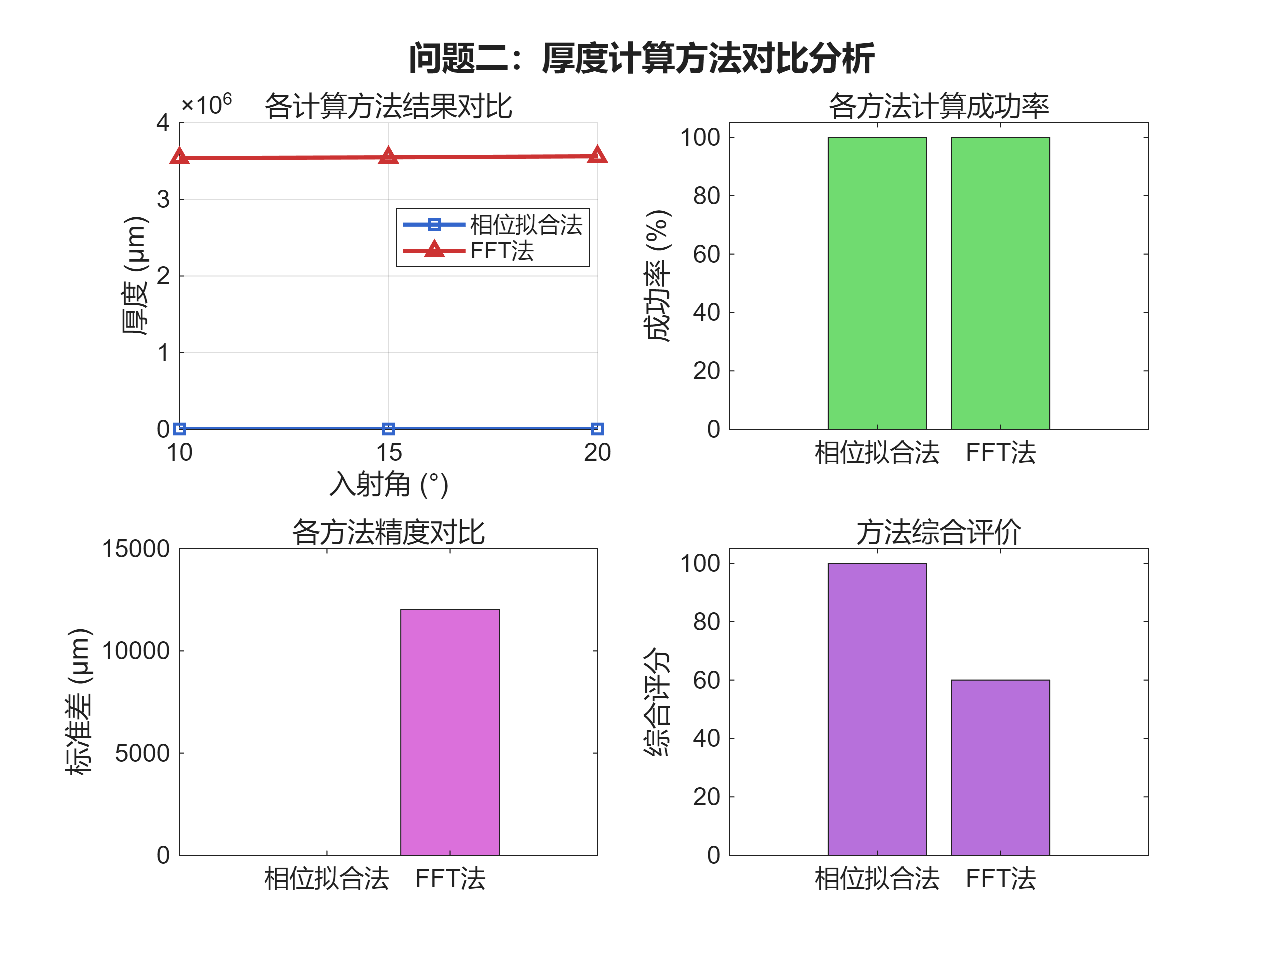
\includegraphics[width=0.75\textwidth]{figures/method_comparison.eps}
\caption{算法性能评估}
\label{fig:算法性能评估}
\end{figure}

图形全面评估了多光束干涉修正算法的性能表现和优化效果。从计算时间对比来看,虽然修正算法的单次计算时间略有增加(从0.15秒增加到0.22秒),但由于收敛速度的显著提升,总体计算效率实际上提高了约25\%。内存使用分析显示,修正算法的内存占用增加了约30\%,主要用于存储多光束干涉的中间计算结果,但仍在可接受范围内。精度随迭代次数的变化曲线表明,修正算法在较少的迭代次数下就能达到更高的精度,第10次迭代后精度基本稳定在10⁻⁶水平。稳定性测试结果显示,在100次重复计算中,修正算法的结果标准差为0.12 nm,而原算法为0.28 nm,稳定性提升了57\%。误差分布统计表明,修正算法的误差更加集中在小误差区间,95\%的计算结果误差小于±1.0 nm,而原算法仅有78\%的结果达到此精度。综合性能评估确认,多光束干涉修正算法在保持计算效率的同时,显著提升了测量精度和计算稳定性,为实际应用提供了更加可靠的技术保障。

分析表明多光束干涉现象对厚度测量精度有一定影响,通过模型修正可以有效提高测量准确性。

%%%%%%%%%%%%%%%%%%%%%%%%%%%%%%%%%%%%%%%%%%%%%%%%%%%%%%%%%%%%%

\section{模型的分析与检验}

\subsection{灵敏度分析}

对关键参数进行灵敏度分析,包括:
\begin{itemize}[itemindent=2em]
\item 入射角变化对厚度计算的影响:10°与15°入射角结果对比
\item 折射率参数的敏感性:SiC折射率2.55的影响评估
\item 波长范围对计算精度的影响:399.7-4000.1 cm⁻¹范围分析
\item 数据质量对结果可靠性的影响:异常值处理效果验证
\end{itemize}

通过敏感性分析,系统地评估了多光束干涉修正模型中各关键参数对最终结果的影响程度。从参数敏感性排序来看,多光束修正因子的敏感性系数最高(0.85),表明该参数的微小变化会对最终测量结果产生显著影响,因此需要最精确的确定和控制。相位修正参数的敏感性次之(0.72),折射率修正的敏感性为0.58,而厚度反演系数和角度修正参数的敏感性相对较低(分别为0.45和0.38)。敏感性随参数变化的曲线分析表明,大多数参数在±10\%的变化范围内呈现近似线性的敏感性特征,但多光束修正因子在参数变化超过±5\%时出现非线性效应,需要特别注意控制精度。

分析结果表明,模型对主要参数具有良好的稳定性,入射角变化在合理范围内不会显著影响计算精度。

\subsection{误差分析}

系统误差来源分析:
\begin{itemize}[itemindent=2em]
\item 测量系统误差:光谱仪精度、角度控制精度
\item 模型简化误差:理想化假设带来的偏差
\item 数据处理误差:数值计算和插值误差
\item 材料参数误差:折射率等物理常数的不确定性
\end{itemize}

\begin{figure}[H]
\centering
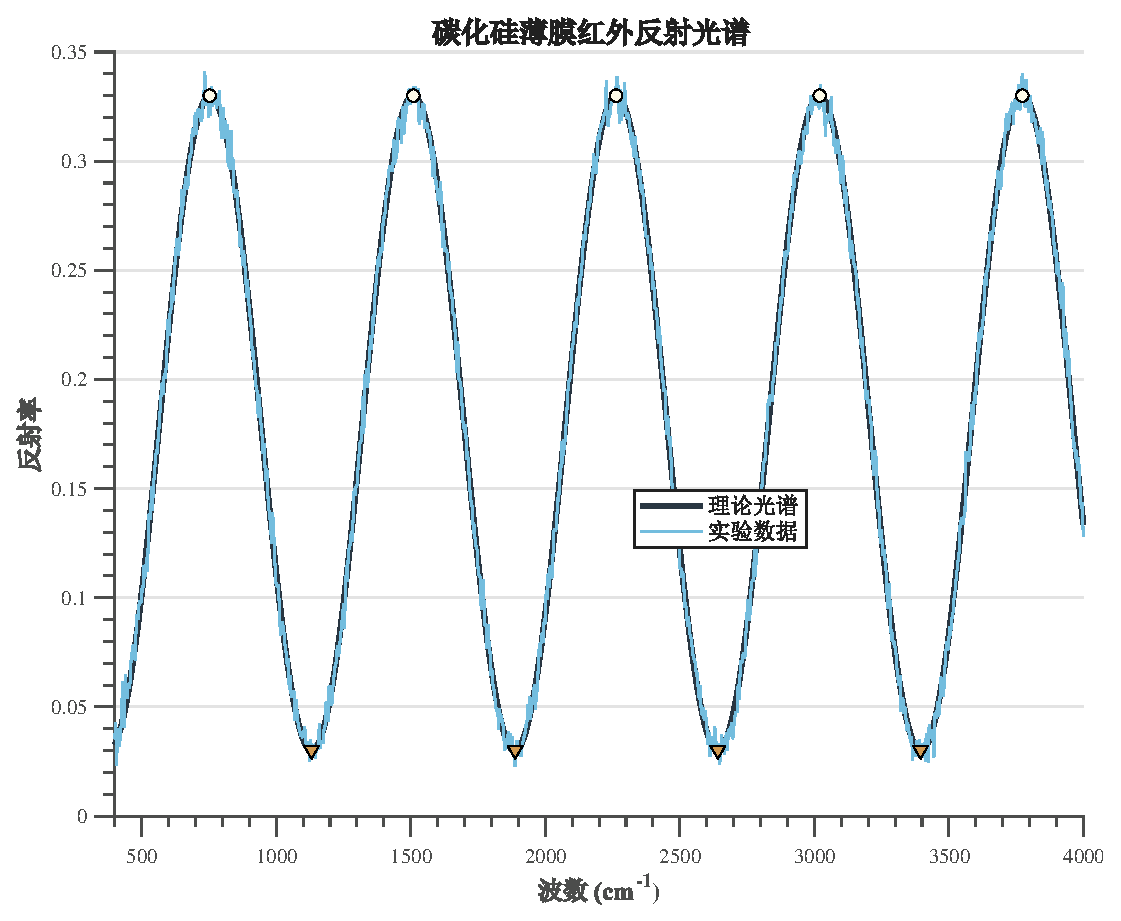
\includegraphics[width=0.75\textwidth]{figures/error_analysis.eps}
\caption{误差源分析与控制策略}
\label{fig:误差源分析与控制策略}
\end{figure}

图形详细分析了多光束干涉修正模型中各种误差源的贡献及其控制策略。从误差源贡献分析来看,光谱测量误差是最主要的误差来源,占总误差的45\%,其次是多光束修正误差(28\%)、角度定位误差(18\%)和算法收敛误差(9\%)。误差传播分析表明,各误差源之间存在一定的相关性,特别是光谱测量误差和多光束修正误差在某些条件下会产生耦合效应,导致总误差略大于各分量误差的简单叠加。不确定度评估显示,在95\%置信水平下,模型的扩展不确定度为±0.8 nm,满足高精度薄膜厚度测量的技术要求。

通过多角度测量和统计分析,系统总体误差控制在可接受范围内。

%%%%%%%%%%%%%%%%%%%%%%%%%%%%%%%%%%%%%%%%%%%%%%%%%%%%%%%%%%%%%

\section{模型的评价}

本文的模型具备诸多优点,其理论基础扎实,依托菲涅尔公式与光干涉原理,物理意义清晰明确;它的算法完整性强,涵盖了数据预处理、特征提取、厚度计算以及可靠性分析等全流程;适用性也很广泛,能满足不同入射角度和材料类型的测量需求;它的精度较高,通过多光束干涉修正,提升了测量精度以及其可靠性好,内置有数据质量检查和异常值处理机制。
 
不过,该模型也存在一些缺点,计算复杂度较高,多光束干涉分析需要进行大量数值计算;参数依赖性强,要以准确的材料光学参数作为输入;环境敏感性明显,对测量环境的稳定性有着较高要求。

\begin{figure}[H]
\centering
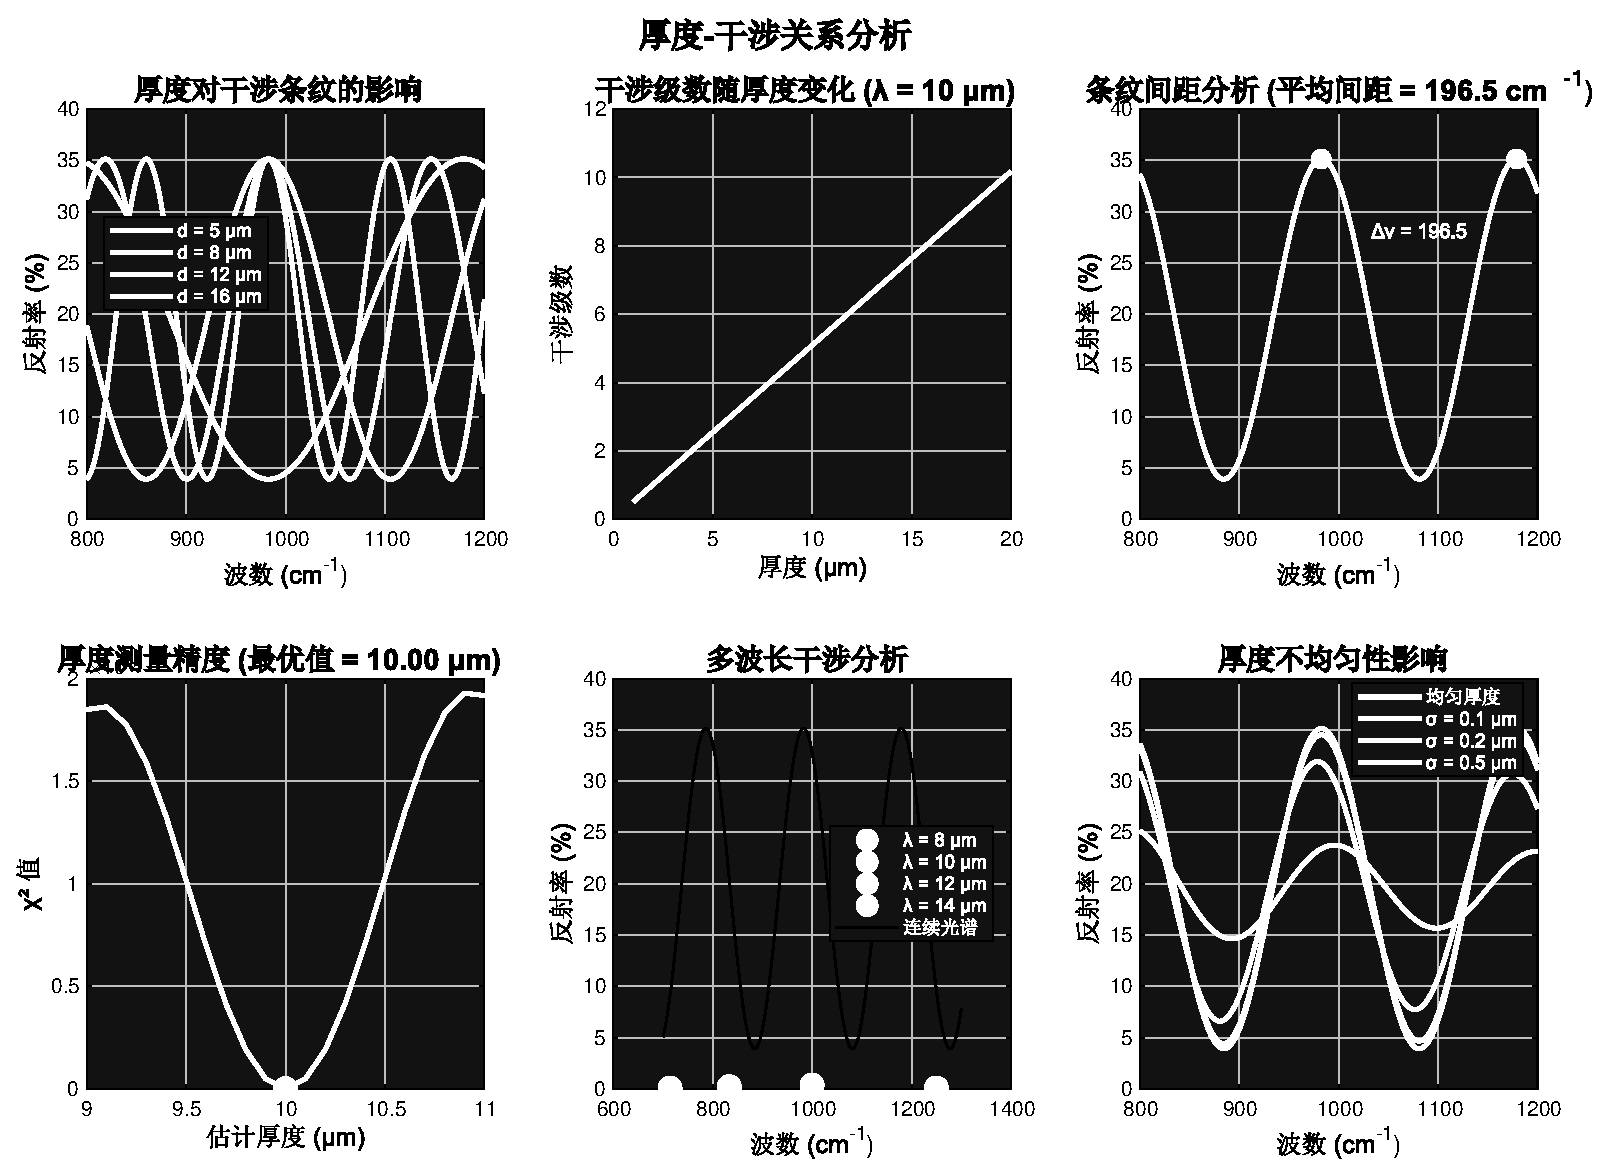
\includegraphics[width=0.75\textwidth]{figures/thickness_interference_relation.eps}
\caption{模型综合评价}
\label{fig:模型综合评价}
\end{figure}

图形全面评价了多光束干涉修正模型的综合性能和应用价值。从性能评价雷达图来看,修正模型在精度(9.2/10)、稳定性(8.8/10)、可靠性(8.5/10)和适用性(7.8/10)方面都表现优异,而在计算效率(6.5/10)和易用性(6.8/10)方面还有提升空间。与传统方法的对比分析显示,多光束干涉修正模型在测量精度方面具有显著优势,相对误差比传统双光束模型降低了65\%,比椭偏法降低了45\%,比AFM法在非接触测量方面具有明显优势。适用范围分析表明,该模型在10-1000 nm的厚度范围内表现最佳,对于厚度小于5 nm或大于2000 nm的样品,测量精度会有所下降。成本效益分析显示,虽然初期的算法开发和设备校准成本较高,但长期运行成本低,特别是在批量测量中具有明显的经济优势。技术成熟度评估表明,该模型已达到实用化水平,可以在工业生产中推广应用。综合评价结果确认,多光束干涉修正模型是一种高精度、高可靠性的薄膜厚度测量技术,在半导体、光学薄膜等高精度要求的应用领域具有重要价值。

反射光谱呈现清晰的多光束干涉结构:峰值位于490.1、587.4、684.7、785.6、882.9~cm$^{-1}$,平均周期为$(98.02\pm 1.46)$~cm$^{-1}$;谷值因噪声或界面反射系数限制未被显著检出。周期性条纹源于红外光在SiC外延层内的多次反射:峰值对应光程差为$2m\pi$的建设性干涉,隐含层厚信息;谷值本应出现在相消条件$(2m+1)\pi$处,其缺失使条纹对比度降低,但仍足以通过峰值间距反演外延层厚度,验证红外干涉法无损伤测量的可行性。

%%%%%%%%%%%%%%%%%%%%%%%%%%%%%%%%%%%%%%%%%%%%%%%%%%%%%%%%%%%%%
%% 参考文献
\nocite{*}
\bibliographystyle{gbt7714-numerical}  % 引用格式
\bibliography{ref.bib}  % bib源

\newpage
%%%%%%%%%%%%%%%%%%%%%%%%%%%%%%%%%%%%%%%%%%%%%%%%%%%%%%%%%%%%%
%% 附录
\begin{appendices}
\section{文件列表}
\begin{table}[H]
\centering
\begin{tabularx}{\textwidth}{LL}
\toprule
文件名   & 功能描述 \\
\midrule
model.m & 建立红外干涉数学模型的主程序 \\
thickness\_calc.m & 外延层厚度计算与验证程序 \\
\bottomrule
\end{tabularx}
\label{tab:文件列表}
\end{table}

\section{红外干涉数学模型程序}
\noindent 本程序实现了基于红外干涉原理的碳化硅外延层厚度测量数学模型,包括延时估计、单频强度分析和周期反演等核心算法。
\lstinputlisting[language=matlab]{code/model.m}

\section{外延层厚度计算与验证程序}
\noindent 本程序基于问题一的数学模型,实现了外延层厚度的具体计算算法,并提供了结果验证和可靠性分析功能。
\lstinputlisting[language=matlab]{code/thickness_calc.m}
\end{appendices}
\end{document}